\documentclass{article}
\include{includes.tex}

\title{Teoría de la Información}
\date{Curso 2023 - 2024}
\author{Lucas Goiriz Beltrán\\ Instituto de Biología Integrativa de Sistemas\\(I$_2$SysBio; UV-CSIC)\\Departamento de Matemática Aplicada\\Universitat Politècnica de València (UPV)}

\begin{document}
\maketitle

\tableofcontents

\pagebreak

\section{Teoría de la Información}\label{teoruxeda-de-la-informaciuxf3n}

% \subsection{Índice}\label{uxedndice}

% \begin{enumerate}
% \def\labelenumi{\arabic{enumi}.}
% \tightlist
% \item
%   \hyperref[introducciuxf3n]{Introducción}
% \item
%   \href{./2-entropia/README.md}{Entropía}
% \item
%   \href{./3-estructura_lenguaje/README.md}{Estructura del lenguaje}
% \item
%   \href{./4-fuentes_informacion/README.md}{Fuentes de Información}
% \end{enumerate}

\subsection{Introducción}\label{introducciuxf3n-teoria-informacion}

La teoría de la información es una rama de las matemáticas que estudia
la cuantificación de la información. Fue propuesta por Claude Shannon en
1948 para estudiar la transmisión de mensajes en sistemas de
comunicación, y desde entonces se ha convertido en una disciplina
fundamental en la ingeniería de la comunicación y en la teoría de la
computación.

La teoría de la información se basa en la teoría de la probabilidad y en
la teoría de los sistemas de comunicación. Su objetivo es estudiar la
cantidad de información que se puede transmitir a través de un canal de
comunicación, y las limitaciones teóricas y prácticas que existen para
la transmisión de información.

\subsubsection{Esquema general de los sistemas de
comunicación}\label{esquema-general-de-los-sistemas-de-comunicaciuxf3n}

\begin{figure}[htbp!]
\centering
\includesvg{./img/shannon_communication_system.svg}
\end{figure}

En general, un sistema de comunicación consta de los siguientes
elementos:

\begin{itemize}
\tightlist
\item
  \textbf{Fuente de información}: es el origen de los mensajes que se
  van a transmitir. Puede ser un ser humano, un sensor, un ordenador,
  etc.
\item
  \textbf{Codificador}: es el encargado de transformar los mensajes de
  la fuente en una forma adecuada para su transmisión a través del canal
  de comunicación.
\item
  \textbf{Canal de comunicación}: es el medio físico a través del cual
  se transmiten los mensajes. Puede ser un cable, una fibra óptica, el
  aire, etc.
\item
  \textbf{Decodificador}: es el encargado de transformar los mensajes
  recibidos a través del canal en una forma adecuada para su
  interpretación por el destinatario.
\item
  \textbf{Destinatario}: es el receptor de los mensajes transmitidos por
  el sistema de comunicación.
\item
  \textbf{Ruido}: es cualquier perturbación que afecta a la transmisión
  de los mensajes a través del canal de comunicación.
\end{itemize}

Es debido a la presencia de ruido en el canal de comunicación que no es
posible transmitir información de forma perfecta. Por ese motivo, es
importante cuantificar la cantidad de información que se puede
transmitir a través de un canal de comunicación, y estudiar las
limitaciones teóricas y prácticas que existen para la transmisión de
información.


\subsection{Entropía}\label{entropuxeda}

\subsubsection{Preliminares}\label{preliminares}

\paragraph{Variable aleatoria}\label{variable-aleatoria}

Una variable aleatoria es una función que asigna un valor numérico a
cada resultado de un experimento aleatorio. Por ejemplo, si lanzamos un
dado, la variable aleatoria \(X\) que representa el número que sale en
la cara superior del dado, puede tomar los valores \(1, 2, 3, 4, 5, 6\).
En ese caso escribiríamos que

\[
X = \{1,2,3,4,5,6\}
\]

Osea, \(X\) es una variable aleatoria que toma valores en el conjunto
\(\{1,2,3,4,5,6\}\).

En el ejemplo anterior, la variable aleatoria \(X\) es discreta, porque
toma valores en un conjunto finito o numerable (recuerda, hay infinitos
más grandes que otros. Un infinito numerable es aquel que se puede poner
en correspondencia con los números naturales \(\mathbb{N}\)). Pero
también hay variables aleatorias continuas, que toman valores en un
intervalo de números reales. Por ejemplo, si medimos la altura de una
persona, la variable aleatoria que representa la altura puede tomar
cualquier valor en el intervalo \((0,\infty)\).

\paragraph{Función de probabilidad}\label{funciuxf3n-de-probabilidad}

La función de probabilidad de una variable aleatoria es una función que
asigna a cada valor de la variable aleatoria la probabilidad de que ese
valor ocurra. Por ejemplo, si lanzamos un dado, la función de
probabilidad de la variable aleatoria \(X\) que representa el número que
sale en la cara superior del dado, es una función que asigna a cada
número del conjunto \(\{1,2,3,4,5,6\}\) la probabilidad de que salga ese
número. En este caso, la función de probabilidad es uniforme, porque
todos los números tienen la misma probabilidad de salir.

Para una variable aleatoria discreta, la función de probabilidad se
puede representar mediante una tabla o mediante una fórmula. Por
ejemplo, si lanzamos un dado, la función de probabilidad de la variable
aleatoria \(X\) que representa el número que sale en la cara superior
del dado, se puede representar mediante la siguiente tabla:

\begin{longtable}[]{@{}ll@{}}
\toprule\noalign{}
\(x\) & \(P(X=x)\) \\
\midrule\noalign{}
\endhead
\bottomrule\noalign{}
\endlastfoot
1 & 1/6 \\
2 & 1/6 \\
3 & 1/6 \\
4 & 1/6 \\
5 & 1/6 \\
6 & 1/6 \\
\end{longtable}

O mediante la siguiente fórmula:

\[
P(X=x) = \frac{1}{6} \quad \text{para } x \in \{1,2,3,4,5,6\}
\]

Para una variable aleatoria continua, la función de probabilidad se
puede representar mediante una función de densidad de probabilidad. Por
ejemplo, si medimos la altura de una persona, la función de densidad de
probabilidad de la variable aleatoria que representa la altura, es una
función que asigna a cada valor del intervalo \((0,\infty)\) la
probabilidad de que la altura de una persona esté en ese intervalo.

\paragraph{Esperanza matemática}\label{esperanza-matemuxe1tica}

La esperanza matemática de una variable aleatoria es el valor promedio
que toma la variable aleatoria en un experimento aleatorio. Se calcula
multiplicando cada valor de la variable aleatoria por su probabilidad, y
sumando los resultados:

\[
\mathbb{E}[X] = \sum_{i=0}^n x_i \cdot P(X=x_i)
\]

Por ejemplo, si lanzamos un dado, la esperanza matemática de la variable
aleatoria \(X\) que representa el número que sale en la cara superior
del dado, se calcula como

\[
\mathbb{E}[X] = 1 \cdot \frac{1}{6} + 2 \cdot \frac{1}{6} + 3 \cdot \frac{1}{6} + 4 \cdot \frac{1}{6} + 5 \cdot \frac{1}{6} + 6 \cdot \frac{1}{6} = 3.5
\]

Osea, en promedio, el número que sale en la cara superior del dado es
3.5.

Para una variable aleatoria continua, la esperanza matemática se calcula
de forma similar, pero en lugar de sumar los valores de la variable
aleatoria, se integran:

\[
\mathbb{E}[X] = \int_{-\infty}^{\infty} xf(x)dx
\]

Donde \(f(x)\) es la función de densidad de probabilidad de la variable
aleatoria \(X\).

\paragraph{\texorpdfstring{LOTUS: \emph{Law of the Unconscious
Statistician} (Ley del Estadístico
Inconsciente)}{LOTUS: Law of the Unconscious Statistician (Ley del Estadístico Inconsciente)}}\label{lotus-law-of-the-unconscious-statistician-ley-del-estaduxedstico-inconsciente}

La LOTUS es una regla que permite calcular la esperanza matemática de
una función de una variable aleatoria, sin necesidad de conocer la
función de probabilidad de la variable aleatoria. La LOTUS establece que
la esperanza matemática de una función de una variable aleatoria se
calcula multiplicando la función por la función de probabilidad de la
variable aleatoria, y sumando los resultados:

\[
\mathbb{E}[g(X)] = \sum_{i=0}^n g(x_i) \cdot P(X=x_i)
\]

Por ejemplo, si lanzamos un dado, y definimos la variable aleatoria
\(Y = X^2\), donde \(X\) es la variable aleatoria que representa el
número que sale en la cara superior del dado, la esperanza matemática de
la variable aleatoria \(Y\) se calcula como

\[
\mathbb{E}[Y] = 1^2 \cdot \frac{1}{6} + 2^2 \cdot \frac{1}{6} + 3^2 \cdot \frac{1}{6} + 4^2 \cdot \frac{1}{6} + 5^2 \cdot \frac{1}{6} + 6^2 \cdot \frac{1}{6} = 15.1667
\]

Osea, en promedio, el cuadrado del número que sale en la cara superior
del dado es 15.1667.

Para una variable aleatoria continua, la LOTUS se calcula de forma
similar, pero en lugar de sumar los valores de la variable aleatoria, se
integran:

\[
\mathbb{E}[g(X)] = \int_{-\infty}^{\infty} g(x)f(x)dx
\]

Donde \(f(x)\) es la función de densidad de probabilidad de la variable
aleatoria \(X\).

\subsubsection{Entropía}\label{entropuxeda-1}

En física, la entropía es una medida de la cantidad de desorden o caos
en un sistema; más concretamente en termodinámica, la entropía es una
medida de la cantidad de energía que no se puede utilizar para realizar
trabajo. En teoría de la información, la entropía es una medida de la
incertidumbre de una variable aleatoria. También se puede interpretar
como una medida de la cantidad de información que se necesita para
describir una variable aleatoria.

La entropía de una variable aleatoria \(X\) se define como la esperanza
matemática de la información de la variable aleatoria. La información de
una variable aleatoria es una medida de la ``\emph{sorpresa}'' que
produce un valor de la variable aleatoria.

La información de una variable aleatoria se calcula como el negativo del
logaritmo de la probabilidad de que ocurra un valor de la variable
aleatoria:

\[
I(x) = -\log_n\left(P(X=x)\right)
\]

Nótese que la base del logaritmo determina la unidad de medida de la
información. Esta base puede ser cualquier número positivo, pero las
bases más comunes son:

\begin{itemize}
\tightlist
\item
  \texttt{2}: en cuyo caso la unidad de medida de la información es el
  \emph{bit} (binary digit).
\item
  \texttt{e}: en cuyo caso la unidad de medida de la información es el
  \emph{nat} (natural unit of information).
\item
  \texttt{10}: en cuyo caso la unidad de medida de la información es el
  \emph{hartley}.
\end{itemize}

\textbf{En caso de no especificar ninguna base, asumiremos que la base
del logaritmo es 2.}

Sabiendo esto, la entropía de una variable aleatoria \(X\), que
denotaremos como \(H_k(X)\), se calcula de la siguiente manera (gracias
al teorema LOTUS):

\[
H_k(X) = \mathbb{E}[I(X)] = \sum_{i=0}^n -\log_k\left(P(X=x_i)\right) \cdot P(X=x_i)
\]

O para una variable aleatoria continua:

\[
H_k(X) = \int_{-\infty}^{\infty} -\log_k\left(f(x)\right) \cdot f(x)dx
\]

donde el subíndice \(k\) indica la base del logaritmo. \textbf{Recordad
que si no se especifica ninguna base, asumiremos que la base del
logaritmo es 2.}

En teoría de la información, partiremos de una fuente de información
definida como un par \((S,P)\) donde \(S\) es un alfabeto predefinido y
\(P\) es una distribución de probabilidad sobre \(S\).

Dado que la fuente de información introduce una incertidumbre en la
variable aleatoria definida por el alfabeto predefinido, la entropía nos
será de utilidad para medir el grado de incertidumbre, el grado de
aleatoriedad en la fuente de información y, en consecuencia, estimar las
unidades de información necesarias en promedio para codificar todos los
valores posibles que puedan darse en la fuente de información.

Debido a las propiedades del logaritmo, \(H_k(X)\) admite las siguientes
definiciones alternativas (pero equivalentes):

\begin{itemize}
\tightlist
\item
  \(H_k(X) = -\sum_{i=0}^n\log_k\left(P(X=x_i)\right)\cdot P(X=x_i)\)
\item
  \(H_k(X) = \sum_{i=0}^n \log_k\left(\frac{1}{P(X=x_i)}\right)P(X=x_i)\)
\end{itemize}

Además, debido a las propiedades del logaritmo (en particular que
\(\log_a(b)=\frac{\log_c(b)}{\log_c(a)}\)), se cumple que
\(H_b(X)=\log_b(a)\cdot H_a(X)\). La demostración es sencilla:


\begin{align*}
H_b(X) &= \sum_{i=0}^n -\log_b\left(P(X=x_i)\right) \cdot P(X=x_i) \\
&= \sum_{i=0}^n -\frac{\log_a\left(P(X=x_i)\right)}{\log_a(b)} \cdot P(X=x_i) \\
&= \frac{1}{\log_a(b)}\sum_{i=0}^n -\log_a\left(P(X=x_i)\right) \cdot P(X=x_i) \\
&= \left(\frac{1}{\log_a(b)}\right)H_a(X) \\
&= \left(\frac{1}{\frac{\log_b(b)}{\log_b(a)}}\right)H_a(X) \\
&= \left(\frac{1}{\frac{1}{\log_b(a)}}\right)H_a(X) \\
&= \log_b(a)\cdot H_a(X) \\
\end{align*}

\begin{center}\rule{0.5\linewidth}{0.5pt}\end{center}

\paragraph{Ejemplo 1: Entropía de una variable aleatoria
discreta}\label{ejemplo-1-entropuxeda-de-una-variable-aleatoria-discreta}

\emph{Sea el alfabeto \(S=\left\{a,b,c,d\right\}\) con una distribución
de probabilidades
\(P=\left\{\frac{1}{2},\frac{1}{4},\frac{1}{8},\frac{1}{8}\right\}\). La
entropía de la variable aleatoria \(X\) definida por el alfabeto \(S\) y
la distribución de probabilidad \(P\) es:}

\[
H(X) = -\left(\frac{1}{2}\log\left(\frac{1}{2}\right) + \frac{1}{4}\log\left(\frac{1}{4}\right) + \frac{1}{8}\log\left(\frac{1}{8}\right) + \frac{1}{8}\log\left(\frac{1}{8}\right)\right) = 1.75
\]

La entropia de la variable aleatoria \(X\) es 1.75 bits.

\begin{center}\rule{0.5\linewidth}{0.5pt}\end{center}

Una propiedad interesante de la entropía es la siguiente: sea \(X\) una
variable aleatoria sobre el alfabeto
\(\left\{x_1,x_2,\dots,x_n\right\}\), entonces:

\[
0 \leq H(X) \leq \log(n)
\]

La entropía de una variable aleatoria \(X\) está acotada por \(0\) y
\(\log(n)\), donde \(n\) es el número de elementos del alfabeto de la
variable aleatoria. La entropía es máxima cuando la distribución de
probabilidad es uniforme, y es mínima cuando la distribución de
probabilidad es degenerada (es decir, cuando un único valor del alfabeto
tiene probabilidad 1 y el resto de valores tienen probabilidad 0).

\begin{center}\rule{0.5\linewidth}{0.5pt}\end{center}

\paragraph{Ejemplo 2: Entropía de una variable aleatoria distribuida
bernoulli}\label{ejemplo-2-entropuxeda-de-una-variable-aleatoria-distribuida-bernoulli}

\emph{Sea \(X\) una variable aleatoria distribuida Bernoulli con
parámetro \(p\) (es decir, \(X\sim\text{Bernoulli}(p)\), lo cual quiere
decir que nuestra variable aleatoria mide ``el número de éxitos en un
experimento de Bernoulli''). La función de probabilidad de \(X\) es:}

\[
P(X=x) = p^x(1-p)^{1-x} \quad \text{para } x\in\{0,1\}
\]

\emph{La entropía de la variable aleatoria \(X\) es:}


\begin{align*}
H(X) &= -\sum_{x=0}^1 p^x(1-p)^{1-x}\log\left(p^x(1-p)^{1-x}\right) \\
&= -\left(p\log(p) + (1-p)\log(1-p)\right) \\
&= (p-1)\log(1-p) -p\log(p)
\end{align*}

Si representamos la entropía de la variable aleatoria \(X\) en función
de \(p\), obtenemos la siguiente gráfica:

\begin{figure}[htbp!]
\centering
\includegraphics[width=0.65\linewidth]{./img/bernoulli_entropy.png}
\end{figure}

\emph{¿Qué interpretación tiene esto?} La entropía de una variable
aleatoria Bernoulli es máxima cuando \(p=0.5\), es decir, cuando la
distribución de probabilidad es uniforme. Esto tiene sentido, porque en
una distribución uniforme, todos los valores del alfabeto tienen la
misma probabilidad de ocurrir, y por lo tanto hay más incertidumbre
sobre el valor que tomará la variable aleatoria. Por otro lado, la
entropía de una variable aleatoria Bernoulli es mínima cuando \(p=0\) o
\(p=1\), es decir, cuando la distribución de probabilidad es degenerada.
Esto también tiene sentido, porque en una distribución degenerada, solo
un valor del alfabeto tiene probabilidad 1 y el resto de valores tienen
probabilidad 0, y por lo tanto no hay incertidumbre sobre el valor que
tomará la variable aleatoria.

\emph{¿Cómo se programaría esto en \texttt{python}?}

\begin{Shaded}
\begin{Highlighting}[]
\ImportTok{import}\NormalTok{ numpy }\ImportTok{as}\NormalTok{ np}
\ImportTok{import}\NormalTok{ matplotlib.pyplot }\ImportTok{as}\NormalTok{ plt}

\KeywordTok{def}\NormalTok{ H\_Bernoulli(p):}

\NormalTok{    h }\OperatorTok{=}\NormalTok{ (p }\OperatorTok{{-}} \DecValTok{1}\NormalTok{)}\OperatorTok{*}\NormalTok{np.log2(}\DecValTok{1} \OperatorTok{{-}}\NormalTok{ p) }\OperatorTok{{-}}\NormalTok{ p}\OperatorTok{*}\NormalTok{np.log2(p)}
    
    \CommentTok{\# Fix the NaN values that occur due to the logarithm of zero}
\NormalTok{    h[np.isnan(h)] }\OperatorTok{=} \DecValTok{0}

    \ControlFlowTok{return}\NormalTok{ h}

\NormalTok{plt.figure(figsize}\OperatorTok{=}\NormalTok{(}\DecValTok{8}\NormalTok{, }\DecValTok{6}\NormalTok{))}

\NormalTok{p }\OperatorTok{=}\NormalTok{ np.linspace(}\DecValTok{0}\NormalTok{, }\DecValTok{1}\NormalTok{, }\DecValTok{200}\NormalTok{)}
\NormalTok{plt.plot(p, H\_Bernoulli(p), }\StringTok{"r"}\NormalTok{, linewidth}\OperatorTok{=}\DecValTok{3}\NormalTok{)}

\NormalTok{plt.grid()}
\NormalTok{plt.xlim(}\DecValTok{0}\NormalTok{, }\DecValTok{1}\NormalTok{)}
\NormalTok{plt.ylim(}\DecValTok{0}\NormalTok{, }\FloatTok{1.005}\NormalTok{)}
\NormalTok{plt.ylabel(}\VerbatimStringTok{r"$H(X)$ (bits)"}\NormalTok{, fontsize}\OperatorTok{=}\DecValTok{16}\NormalTok{)}
\NormalTok{plt.xlabel(}\VerbatimStringTok{r"$p$"}\NormalTok{, fontsize}\OperatorTok{=}\DecValTok{16}\NormalTok{)}
\NormalTok{plt.tick\_params(axis}\OperatorTok{=}\StringTok{"both"}\NormalTok{, which}\OperatorTok{=}\StringTok{"major"}\NormalTok{, labelsize}\OperatorTok{=}\DecValTok{14}\NormalTok{)}
\end{Highlighting}
\end{Shaded}

\paragraph{Recordatorio: probabilidades conjuntas y
condicionales}\label{recordatorio-probabilidades-conjuntas-y-condicionales}

Dadas dos variables aleatorias \(X\) e \(Y\), la probabilidad conjunta
de \(X\) e \(Y\) es la probabilidad de que ambas variables aleatorias
tomen un valor determinado. Se denota como \(P(X=x,Y=y)\), y se calcula
de la siguiente manera:

\[
P(X=x,Y=y) = P(Y=y|X=x)P(X=x)
\]

donde \(P(Y=y|X=x)\) es la probabilidad condicional de \(Y\) dado \(X\),
es decir, la probabilidad de que \(Y\) tome un valor determinado dado
que \(X\) ha tomado un valor determinado.

De la misma manera, podemos definir la probabilidad conjunta como

\[
P(X=x,Y=y) = P(X=x|Y=y)P(Y=y)
\]

Igualando ambas expresiones, se obtiene el Teorema de Bayes:

\[
P(Y=y|X=x) = \frac{P(X=x|Y=y)P(Y=y)}{P(X=x)}
\]

Además, si las variables aleatorias \(X\) e \(Y\) son independientes,
entonces la probabilidad conjunta de \(X\) e \(Y\) es igual al producto
de las probabilidades marginales de \(X\) e \(Y\):

\[
P(X=x,Y=y) = P(X=x)P(Y=y)
\]

¿Por qué? Porque si \(X\) e \(Y\) son independientes, entonces la
probabilidad de que \(Y\) tome un valor determinado no depende de que
\(X\) haya tomado un valor determinado, y viceversa, por ende
\(P(Y=y|X=x) = P(Y=y)\) y \(P(X=x|Y=y) = P(X=x)\).

\paragraph{Entropía conjunta y entropía
condicional}\label{entropuxeda-conjunta-y-entropuxeda-condicional}

Hasta ahora hemos definido la entropía de una única variable aleatoria.
Pero en muchos problemas de teoría de la información, estamos
interesados en la entropía de dos o más variables aleatorias.

La entropía conjunta de dos variables aleatorias \(X\) e \(Y\) se define
como la entropía de la variable aleatoria \((X,Y)\), que es una variable
aleatoria que toma valores en el producto cartesiano (es decir, todas
las parejas posibles) de los alfabetos de \(X\) e \(Y\). La entropía
conjunta de \(X\) e \(Y\) se denota como \(H(X,Y)\), y se calcula de la
siguiente manera:

\[
H(X,Y) = -\sum_{x\in S_X}\sum_{y\in S_Y} P(X=x,Y=y)\log\left(P(X=x,Y=y)\right)
\]

O para variables aleatorias continuas:

\[
H(X,Y) = -\int_{-\infty}^{\infty}\int_{-\infty}^{\infty} f(x,y)\log\left(f(x,y)\right)dxdy
\]

Otra manera de escribir la entropía conjunta sería utilizando índices
para los valores de las variables aleatorias:

\[
H(X,Y) = -\sum_{i=0}^n\sum_{j=0}^m P(X=x_i,Y=y_j)\log\left(P(X=x_i,Y=y_j)\right)
\]

En algunos casos, esta notación es más clara que la notación con los
alfabetos \(S_X\) y \(S_Y\). Habitualmente \(S_X = S_Y\), es decir,
estamos usando el mismo alfabeto para ambas variables aleatorias.

De forma similar a la entropía conjunta, podemos definir la entropía
condicional de una variable aleatoria \(X\) dada otra variable aleatoria
\(Y\). La entropía condicional de \(X\) dado \(Y\) se denota como
\(H(X|Y)\), y se calcula de la siguiente manera:

\[
H(X|Y) = -\sum_{x\in S_X}\sum_{y\in S_Y} P(X=x,Y=y)\log\left(P(X=x|Y=y)\right)
\]

Es más, utilizando las propiedades de las probabilidades conjuntas y
condicionales, podemos escribir la entropía condicional de \(X\) dado
\(Y\) de la siguiente manera:


\begin{align*}
H(X|Y) &= -\sum_{x\in S_X}\sum_{y\in S_Y} P(X=x,Y=y)\log\left(P(X=x|Y=y)\right) \\
&= -\sum_{x\in S_X}\sum_{y\in S_Y} P(X=x|Y=y)P(Y=y)\log\left(P(X=x|Y=y)\right) \\
&= -\sum_{y\in S_Y} P(Y=y)\sum_{x\in S_X} P(X=x|Y=y)\log\left(P(X=x|Y=y)\right) \\
&= \sum_{y\in S_Y} P(Y=y)H(X|Y=y)
\end{align*}


De la misma manera que hemos hecho en la demostración anterior, las
propiedades de la entropia conjunta se originan de operar con las
probabilidades conjuntas y condicionales de las variables aleatorias
\(X\) e \(Y\).

Una de estas propiedades es

\[
H(X,Y) = H(X) + H(Y|X) = H(Y) + H(X|Y)
\]

Esta propiedad se conoce como la regla de la cadena de la entropía, y se
puede demostrar a partir de la definición de la entropía conjunta y
condicional:

\begin{align*}
H(X,Y) &= -\sum_{x\in S_X}\sum_{y\in S_Y} P(X=x,Y=y)\log\left(P(X=x,Y=y)\right) \\
&= -\sum_{x\in S_X}\sum_{y\in S_Y} P(X=x,Y=y)\log\left(P(X=x|Y=y)P(Y=y)\right) \\
&= -\sum_{x\in S_X}\sum_{y\in S_Y} P(X=x,Y=y)\left(\log\left(P(X=x|Y=y)\right) + \log\left(P(Y=y)\right)\right) \\
&= -\sum_{x\in S_X}\sum_{y\in S_Y} P(X=x,Y=y)\log\left(P(X=x|Y=y)\right) - \sum_{x\in S_X}\sum_{y\in S_Y} P(X=x,Y=y)\log\left(P(Y=y)\right) \\
&= H(X|Y) - \sum_{y\in S_Y} P(Y=y)\log\left(P(Y=y)\right) \\
&= H(X|Y) + H(Y)
\end{align*}


De la misma manera, se puede demostrar que \(H(X,Y) = H(Y) + H(X|Y)\).

De este resultado se puede demostrar que dadas las variables aleatorias
\(X\) e \(Y\):

\begin{enumerate}
\def\labelenumi{\arabic{enumi}.}
\tightlist
\item
  \(H(X,Y) \leq H(X) + H(Y)\)
\item
  \(H(X,Y) = H(X) + H(Y)\), (en caso de que \(X\) e \(Y\) sean
  independientes)
\end{enumerate}

\emph{Una forma sencilla de pensar sobre estas propiedades es pensar en
las probabilidades conjuntas y condicionales, de las cuales obtenemos
desigualdades similares, solamente que en el caso de la entropía, debido
al logaritmo, las desigualdades no son productos si no sumas.}

Un corolario de las propiedades anteriores es que:

\begin{enumerate}
\def\labelenumi{\arabic{enumi}.}
\tightlist
\item
  \(H(X|Y) \leq H(X)\)
\item
  \(H(X|Y) = H(X)\), (en caso de que \(X\) e \(Y\) sean independientes)
\end{enumerate}

\begin{center}\rule{0.5\linewidth}{0.5pt}\end{center}

Volviendo a la regla de la cadena, esta la podemos extender para el caso
de más de dos variables, y se define como:

\[
H(X_1,X_2,\dots,X_n) = H(X_1) + H(X_2|X_1) + H(X_3|X_1,X_2) + \dots + H(X_n|X_1,X_2,\dots,X_{n-1})
\]

o de forma más compacta:

\[
H(X_1,X_2,\dots,X_n) = \sum_{i=1}^n H(X_i|X_1,X_2,\dots,X_{i-1})
\]

\paragraph{Entropía Relativa}\label{entropuxeda-relativa}

La entropía relativa, también conocida como divergencia de
Kullback-Leibler, es una medida de la diferencia entre dos
distribuciones de probabilidad (la cantidad de información que se
necesita para describir una distribución de probabilidad utilizando otra
distribución de probabilidad). La entropía relativa de dos
distribuciones de probabilidad \(P\) y \(Q\) se denota como \(D(P||Q)\),
y se calcula de la siguiente manera:

\[
D(P||Q) = \sum_{x\in S} P(x)\log\left(\frac{P(x)}{Q(x)}\right)
\]

O para distribuciones de probabilidad continuas:

\[
D(P||Q) = \int_{-\infty}^{\infty} f(x)\log\left(\frac{f(x)}{g(x)}\right)dx
\]

La entropía relativa es siempre \textbf{no negativa}, y es igual a cero
si y solo si \(P\) y \(Q\) son iguales.

\paragraph{Información Mutua}\label{informaciuxf3n-mutua}

La información mutua de dos variables aleatorias \(X\) e \(Y\) es una
medida de la cantidad de información que una variable aleatoria
proporciona sobre la otra variable aleatoria. La información mutua de
\(X\) e \(Y\) se denota como \(I(X;Y)\), y se calcula de la siguiente
manera:

\[
I(X;Y) = \sum_{x\in S_X}\sum_{y\in S_Y} P(X=x,Y=y)\log\left(\frac{P(X=x,Y=y)}{P(X=x)P(Y=y)}\right)
\]

O para variables aleatorias continuas:

\[
I(X;Y) = \int_{-\infty}^{\infty}\int_{-\infty}^{\infty} f(x,y)\log\left(\frac{f(x,y)}{f(x)f(y)}\right)dxdy
\]

La información mutua es siempre \textbf{no negativa}, y es igual a cero
si y solo si \(X\) e \(Y\) son independientes. Se puede pensar también
que la información mutua es la entropía relativa entre la distribución
conjunta de dos variables aleatorias y el producto de sus distribuciones
marginales.

De la definición de la información mutua se pueden deducir las
siguientes propiedades:

\begin{enumerate}
\def\labelenumi{\arabic{enumi}.}
\tightlist
\item
  \(I(X;Y) = H(X) - H(X|Y) = H(Y) - H(Y|X)\)
\item
  \(I(X;Y) = H(X) + H(Y) - H(X,Y)\)
\item
  \(I(X;Y) = I(Y;X)\)
\item
  \(I(X;X) = H(X)\)
\end{enumerate}

Gráficamente, estas propiedades se pueden representar de la siguiente
manera:

\vspace{-8cm}

\begin{figure}[htbp!]
\centering
\includesvg[width=0.95\linewidth]{./img/mutual_information_relation_diagram.svg}
\end{figure}


\paragraph{El caso contínuo}\label{el-caso-contuxednuo}

\paragraph{Ejemplo 1: Distribución
uniforme}\label{ejemplo-1-distribuciuxf3n-uniforme}

Sea la variable aleatoria \(X\) uniformemente distribuída entre \(0\) y
\(a\). Su función de densidad de probabilidad es

\[
f(x)=\begin{cases}
\frac{1}{a}\quad\text{si }x\in\left[0,a\right]\\
0\quad\text{en caso contrario}
\end{cases}
\]

Su entropía es

\begin{align*}
H(X) &= -\int_{-\infty}^\infty f(x)\log\left(f(x)\right)dx\\
&= -\int_{-\infty}^0 0\log(0)dx - \int_0^a \frac{1}{a}\log\left(\frac{1}{a}\right)dx - \int_0^{\infty} 0\log(0)dx\\
&= \int_0^a \frac{1}{a}\log(a)dx\\
&= \left[\frac{x}{a}\log(a)\right]_0^a\\
&= \log(a)
\end{align*}


\paragraph{Ejemplo 2: Distribución
normal}\label{ejemplo-2-distribuciuxf3n-normal}

Sea la variable aleatoria \(X\) con función de densidad de probabilidad

\[
f(x) = \frac{1}{\sigma\sqrt{2\pi}}e^{\frac{-(x-\mu)^2}{2\sigma^2}}
\]

\emph{(es decir una distribución normal con media \(\mu\) y varianza
\(\sigma^2\))}

Su entropía es


\begin{align*}
H(X) &= -\int_{-\infty}^\infty f(x)\log\left(f(x)\right)dx\\
&= -\int_{-\infty}^\infty \frac{1}{\sigma\sqrt{2\pi}}e^{\frac{-(x-\mu)^2}{2\sigma^2}}\log\left(\frac{1}{\sigma\sqrt{2\pi}}e^{\frac{-(x-\mu)^2}{2\sigma^2}}\right)dx\\
&= -\int_{-\infty}^\infty \frac{1}{\sigma\sqrt{2\pi}}e^{\frac{-(x-\mu)^2}{2\sigma^2}}\left(-\log\left(\sigma\sqrt{2\pi}\right)+\frac{-\log\left(e\right)(x-\mu)^2}{2\sigma^2}\right)dx\\
&= -\left(-\log\left(\sigma\sqrt{2\pi}\right)\int_{-\infty}^\infty \frac{1}{\sigma\sqrt{2\pi}}e^{\frac{-(x-\mu)^2}{2\sigma^2}} + \int_{-\infty}^\infty \frac{-\log\left(e\right)(x-\mu)^2}{2\sigma^3\sqrt{2\pi}}e^{\frac{-(x-\mu)^2}{2\sigma^2}}\right)dx\\
&= -\left(-\log\left(\sigma\sqrt{2\pi}\right)\cdot 1 - \frac{\log\left(e\right)}{2\sigma^2}\int_{-\infty}^\infty \frac{(x-\mu)^2}{\sigma\sqrt{2\pi}}e^{\frac{-(x-\mu)^2}{2\sigma^2}}\right)dx\\
&= \log\left(\sigma\sqrt{2\pi}\right) + \frac{\log\left(e\right)}{2\sigma^2}\left(\sigma^2\right)\\
&= \log\left(\sigma\sqrt{2\pi}\right) + \frac{\log\left(e\right)}{2}\\
&= \log\left(\sigma\sqrt{2\pi}\right) + \log\left(\sqrt{e}\right)\\
&= \log\left(\sigma\sqrt{2\pi e}\right)\\
\end{align*}



\subsection{Estructura del lenguaje}\label{estructura-del-lenguaje}

Antes de estudiar fuentes de información, es necesario definir un
lenguaje para representar los mensajes que se van a transmitir. En
general, un lenguaje es un conjunto de símbolos y reglas que permiten
construir mensajes a partir de esos símbolos.

\subsubsection{Alfabetos y palabras}\label{alfabetos-y-palabras}

Un \textbf{alfabeto} es un conjunto finito de símbolos. Por ejemplo,
nuestro alfabeto podría decirse que está formado por las letras del
abecedario. Un \textbf{símbolo} es un elemento de un alfabeto. Por
ejemplo, la letra ``a'' es un símbolo de nuestro alfabeto.

En lenguaje formal matemático, un alfabeto \(\mathcal{A}\) es un
conjunto finito (salvo que se indique lo contrario de forma explícita) y
no vacío cuyos elementos se denominan \textbf{símbolos}. Por ejemplo, si
\(\mathcal{A} = \{a, b, c\}\), entonces \(a\), \(b\) y \(c\) son
símbolos de \(\mathcal{A}\).

Sea entonces \(\mathcal{A}\) un alfabeto. Una \textbf{palabra} \(x\) es
una secuencia finita de símbolos de \(\mathcal{A}\) de la forma

\[
x=a_1a_2\dots a_n, \quad a_i \in \mathcal{A}, \quad i=1,2,\dots,n
\]

Definimos la \textbf{longitud} de una palabra \(x\) como el número de
símbolos que contiene. La longitud de una palabra \(x\) se denota por
\(|x|\).

Sea \(\mathcal{A}^n,n\geq 1\) el conjunto de todas las palabras de
longitud \(n\) formadas por símbolos de \(\mathcal{A}\).

El número de elementos (también llamado cardinal) de \(\mathcal{A}^n\)
es \(|\mathcal{A}|^n\).

\begin{center}\rule{0.5\linewidth}{0.5pt}\end{center}

\paragraph{Ejemplo}\label{ejemplo}

Tenemos un alfabeto \(\mathcal{A}=\{0,1\}\), y queremos encontrar el
conjunto de todas las palabras de longitud 3 formadas por símbolos de
\(\mathcal{A}\).

Entonces, \(\mathcal{A}^3=\{000,001,010,011,100,101,110,111\}\).

Como \(|\mathcal{A}|=2\), el número de elementos de \(\mathcal{A}^3\) es
\(|\mathcal{A}|^3=2^3=8\).

\begin{center}\rule{0.5\linewidth}{0.5pt}\end{center}

Teniendo un alfabeto \(\mathcal{A}\), el conjunto de todas las palabras
finitas (no nulas) formadas por símbolos de \(\mathcal{A}\) se denota
por \(\mathcal{A}^+\) y se define como:


\begin{align*}
\mathcal{A}^+&=\mathcal{A}^1\cup\mathcal{A}^2\cup\dots\cup\mathcal{A}^n,\quad n\geq1\\
&= \bigcup_{n\geq1}\mathcal{A}^n
\end{align*}


Es decir, \(\mathcal{A}^+\) es la unión de todos los conjuntos de
palabras de longitud \(n\) formadas por símbolos de \(\mathcal{A}\). Se
trata de un conjunto donde existen palabras de todas las longitudes
posibles hasta un máximo de longitud \(n\). Este conjunto se parece un
poco a las palabras en el lenguaje natural, donde existen palabras de
diferentes longitudes.

\emph{¿Cuántos elementos tiene \(\mathcal{A}^+\)?}

Sabemos que


\begin{align*}
\mathcal{A}^+&= \bigcup_{n\geq1}\mathcal{A}^n\\
&=\mathcal{A}^1\cup\mathcal{A}^2\cup\dots\cup\mathcal{A}^n,\quad n\geq1\\
\end{align*}


Además, el número de elementos de \(\mathcal{A}^n\) es
\(|\mathcal{A}|^n\). Por lo tanto, el número de elementos de
\(\mathcal{A}^+\) es


\begin{align*}
|\mathcal{A}^+|&=|\mathcal{A}^1|+|\mathcal{A}^2|+\dots+|\mathcal{A}^n|\\
&=|\mathcal{A}|+|\mathcal{A}|^2+\dots+|\mathcal{A}|^n\\
&=\sum_{n\geq1}|\mathcal{A}|^n
\end{align*}


Esto se parece a una serie geométrica\ldots{}


\begin{align*}
\sum_{n\geq 1}|\mathcal{A}|^n&=\sum_{n\geq 0}|\mathcal{A}|^n - 1\\
&=\frac{1-|\mathcal{A}|^{n+1}}{1-|\mathcal{A}|} - 1\\
\end{align*}


Por lo tanto, el número de elementos de \(\mathcal{A}^+\) es

\[
|\mathcal{A}^+|=\frac{1-|\mathcal{A}|^{n+1}}{1-|\mathcal{A}|} - 1
\]

\begin{center}\rule{0.5\linewidth}{0.5pt}\end{center}

\paragraph{Ejemplo}\label{ejemplo-1}

Tenemos un alfabeto \(\mathcal{A}=\{0,1\}\), y queremos encontrar el
conjunto de todas las palabras finitas (no nulas, de hasta un máximo de
longitud 5) formadas por símbolos de \(\mathcal{A}\). ¿Cuántos elementos
tiene \(\mathcal{A}^+\)?

Sin necesidad de construir cada palabra, podemos calcular el número de
elementos de \(\mathcal{A}^+\) usando la fórmula anterior. Como
\(|\mathcal{A}|=2\) y \(n=5\), el número de elementos de
\(\mathcal{A}^+\) es


\begin{align*}
|\mathcal{A}^+|&=\frac{1-|\mathcal{A}|^{n+1}}{1-|\mathcal{A}|} - 1\\
&=\frac{1-2^{5+1}}{1-2} - 1\\
&=\frac{1-64}{-1} - 1\\
&=62
\end{align*}


\begin{center}\rule{0.5\linewidth}{0.5pt}\end{center}

Para cualquier palabra \(x\in\mathcal{A}^+\) y \(1\leq n\leq|x|\), sea
\(x[n]=a_n\), el \(n\)-ésimo símbolo de la secuencia. Por tanto

\[
x=x[1]\dots x[|x|]
\]

Dadas dos palabras \(x,y\in\mathcal{A}^+\), decimos que \(x\) e \(y\)
son \textbf{iguales} si y solo si:

\[
x = y \Leftrightarrow\begin{cases}
&\left(|x|=|y|\right)\\
&\wedge\left(x[i]=y[i], \forall 1\leq i\leq|x|\right)
\end{cases}
\]

Es decir, son iguales cuando tienen la misma longitud, y además todos
sus símbolos son iguales en la misma posición.

De forma similar, definimos la \textbf{concatenación} de dos palabras
\(x,y\in\mathcal{A}^+\) (que denotaremos como \(xy\)) como la palabra
\(z\in\mathcal{A}^+\) definida por

\begin{enumerate}
\def\labelenumi{\arabic{enumi}.}
\tightlist
\item
  \(|z| = |x| + |y|\)
\item
  \(z[i] = x[i]\) con \(1\leq i\leq|x|\)
\item
  \(z[|x|+i] = y[i]\) con \(1\leq i\leq |y|\)
\end{enumerate}

Es decir, la concatenación de dos palabras es una nueva palabra que
contiene todos los símbolos de la primera palabra seguidos de todos los
símbolos de la segunda palabra.

Es sencillo ver que la concatenación de palabras es una operación
\textbf{asociativa}, es decir, para cualquier \(x,y,z\in\mathcal{A}^+\),
se cumple que

\[
(x y) z = x (y z)
\]

Sin embargo, la concatenación de palabras \textbf{no es conmutativa}, es
decir, en general no se cumple que

\[
xy = yx
\]

\emph{Podéis pensar en esto como si se tratase de ``sumar strings'' en
\texttt{python}\ldots{} Tened cuidado con el sistema de indexación, ya
que en \texttt{python} los índices empiezan en 0, mientras que aquí los
hemos hecho empezar en 1.}

\begin{center}\rule{0.5\linewidth}{0.5pt}\end{center}

En muchas ocasiones es conveniente definir un elemento identidad para
una operación (en este caso, la concatenación de palabras). La identidad
de la concatenación de palabras es la palabra vacía, que denotaremos
como \(\lambda\) (pensad en el string vacío \texttt{""} en
\texttt{python}). \(\lambda\) tiene las siguienets propiedades:

\begin{enumerate}
\def\labelenumi{\arabic{enumi}.}
\tightlist
\item
  \(|\lambda| = 0\)
\item
  \(\mathcal{A}^0 = \left\{\lambda\right\}\)
\item
  \(\forall x\in\mathcal{A}^+,\quad x\neq\lambda\)
\item
  \(|x| = 0 \Leftrightarrow x = \lambda\)
\end{enumerate}

Es decir, que la palabra vacía es la única palabra de longitud 0, y es
la única palabra que no tiene símbolos. Si una palabra tiene longitud 0,
entonces es la palabra vacía, y si una palabra no es la palabra vacía,
entonces tiene longitud mayor que 0.

De esta manera podemos generar otro conjunto, el cual incluye a la
palabra vacía, que denotaremos como \(\mathcal{A}^*\) y se define como


\begin{align*}
\mathcal{A}^* &= \mathcal{A}^+\cup\left\{\lambda\right\}\\
&= \mathcal{A}^+\cup\mathcal{A}^0\\
&= \left(\bigcup_{n\geq1}\mathcal{A}^n\right)\cup\mathcal{A}^0\\
&= \bigcup_{n\geq0}\mathcal{A}^n
\end{align*}


Podemos extender la operación de concatenación de palabras a
\(\mathcal{A}^*\), de manera que para cualquier \(x,y\in\mathcal{A}^*\),
se cumplen las propiedades anteriores de la concatenación, y además

\[
\lambda x = x\lambda = x
\]

Convirtiéndose de esta manera la concatenación de palabras sobre
\(\mathcal{A}^*\) en una operación asociativa y con elemento neutro.

\begin{center}\rule{0.5\linewidth}{0.5pt}\end{center}

A partir de la concatenación de palabras es posible definir la
\textbf{potencia} de una palabra. Dada una palabra \(x\in\mathcal{A}^+\)
y un número entero no negativo \(k\), la potencia de \(x\) elevada a
\(k\), denotada como \(x^k\), se define como

\begin{enumerate}
\def\labelenumi{\arabic{enumi}.}
\tightlist
\item
  \(x^0=\lambda\)
\item
  \(x^k=x^{k-1}x\)
\end{enumerate}

Es decir, la potencia de una palabra es la concatenación de la palabra
consigo misma \(k\) veces.

\begin{center}\rule{0.5\linewidth}{0.5pt}\end{center}

\paragraph{Ejemplo}\label{ejemplo-2}

Dada la palabra \(x=010\), calculamos \(x^3\) como


\begin{align*}
x^3&=x^2x\\
&=(xx)x\\
&=(010010)010\\
&=010010010
\end{align*}


\begin{center}\rule{0.5\linewidth}{0.5pt}\end{center}

Una propiedad que se observa inmediatamente es que
\(\left|x^k\right|=k\left|x\right|\). Es decir, la longitud de la
potencia de una palabra es igual al producto de la longitud de la
palabra por el exponente de la potencia.

Además, otra propiedad es que
\(\forall n>1,\quad x^n = x \Leftrightarrow x = \lambda\). Es decir, que
una palabra elevada a un exponente mayor que 1 es igual a la palabra si
y solo si la palabra es la palabra vacía.

\begin{center}\rule{0.5\linewidth}{0.5pt}\end{center}

También es posible ``\emph{extraer}'' trozos de una palabra. Si tenemos
una palabra \(x\in\mathcal{A}^+\), definimos su segmento \(x[i:j]\) como

\[
x[i:j] =\begin{cases}
& x[i]\dots x[j],\quad 1\leq i\leq j\leq|x|\\
& x[i],\quad 1\leq i = j\leq |x|\\
& \lambda,\quad\text{en otro caso}
\end{cases}
\]

Es decir, que el segmento de una palabra es la subsecuencia de la
palabra que va desde el símbolo \(i\)-ésimo hasta el símbolo
\(j\)-ésimo, ambos incluidos. Si \(i=j\), entonces el segmento es
simplemente el símbolo \(i\)-ésimo, y si \(i>j\), entonces el segmento
es la palabra vacía.

Rápidamente se puede deducir que \(x = x[1:|x|]\). Es decir, que una
palabra es igual a su segmento que va desde el primer símbolo hasta el
último símbolo.

\subsubsection{Órdenes Alfabéticos}\label{uxf3rdenes-alfabuxe9ticos}

Dado un alfabeto \(\mathcal{A}\), es posible definir un \textbf{orden
alfabético} sobre los símbolos de \(\mathcal{A}\). Un orden alfabético
es una relación de orden dada mediante enumeración (sin repetición) de
los símbolos de \(\mathcal{A}\). Si
\(\mathcal{A}=\{a_1,a_2,\dots,a_n\}\), es una enumeración sin
repetición, entonces

\[
a_i < a_j \Leftrightarrow i < j
\]

Es decir, que el orden alfabético de los símbolos de \(\mathcal{A}\) es
el orden de dicha enumeración.

\begin{center}\rule{0.5\linewidth}{0.5pt}\end{center}

Este órden alfabético se puede extender a las palabras de
\(\mathcal{A}^*\) de la siguiente manera. Dadas dos palabras
\(x,y\in\mathcal{A}^+\), decimos que \(x\) es \textbf{menor} que \(y\)
en el orden alfabético si y solo si:

\[
x < y \Leftrightarrow\begin{cases}
& \left(\exists u\in\mathcal{A}^+:y=xu\right)\\
& \vee\left(\exists u,v,w\in\mathcal{A}^*, \exists a,b\in\mathcal{A}:(x=uav
)\wedge (y=ubw) \wedge (a<b)\right)\\
\end{cases}
\]

Es decir, que una palabra es menor que otra en el orden alfabético si y
solo si es un prefijo de la otra palabra, o si ambas palabras tienen un
prefijo común y el siguiente símbolo de una es menor que el siguiente
símbolo de la otra. Nótese que el prefijo común puede ser la palabra
vacía ya que \(\lambda\) es prefijo de cualquier palabra y
\(u,v,w\in\mathcal{A}^*\).

Nótese que trivialmente se tienen las siguientes propiedades:

\begin{enumerate}
\def\labelenumi{\arabic{enumi}.}
\tightlist
\item
  \(\forall x\in\mathcal{A}^+:\lambda < x\)
\item
  \(\forall x,y\in\mathcal{A}^*:x\neq y \Rightarrow ((x<y)\vee(y<x))\)
\item
  Sobre cada alfabeto \(\mathcal{A}\), pueden definirse
  \(\left|\mathcal{A}\right|!\) órdenes alfabéticos distintos.
\end{enumerate}

\begin{center}\rule{0.5\linewidth}{0.5pt}\end{center}

\paragraph{Ejemplo 1}\label{ejemplo-1-1}

Sean las palabras \(x=010\) e \(y=011\). ¿Cuál es la relación de orden
alfabético entre \(x\) e \(y\)?

Para determinar la relación de orden alfabético entre \(x\) e \(y\),
primero comprobamos si \(x\) es prefijo de \(y\) o viceversa. En este
caso, \(x\) no es prefijo de \(y\) y \(y\) no es prefijo de \(x\). Por
tanto, comprobamos si tienen un prefijo común. En este caso, el prefijo
común es la palabra vacía \(\lambda\). Por consiguiente, comprobamos si
el siguiente símbolo de \(x\) es menor que el siguiente símbolo de
\(y\). En este caso, el siguiente símbolo de \(x\) es 1 y el siguiente
símbolo de \(y\) es 1. Como 0 es menor que 1, entonces \(x < y\) en el
orden alfabético.

\begin{center}\rule{0.5\linewidth}{0.5pt}\end{center}

\subsubsection{Prefijos, Sufijos y
Segmentos}\label{prefijos-sufijos-y-segmentos}

Anteriormente hemos definido el segmento de una palabra de forma breve.
Ahora vamos a definir de forma más precisa los conceptos de prefijo,
sufijo y segmento, dado que de forma indirecta hemos utilizado estos
conceptos en la definición de órdenes alfabéticos.

\paragraph{Prefijos}\label{prefijos}

Diremos que para \(x,y\in\mathcal{A}^*\) que \(x\) es un
\textbf{prefijo} de \(y\) siempre que

\[
\exists u\in\mathcal{A}^*:y=xu
\]

Es decir, que una palabra es prefijo de otra si y solo si la otra
palabra es la concatenación de la primera palabra con otra palabra
cualquiera.

Trivialmente, se cumplen las siguientes propiedades:

\begin{enumerate}
\def\labelenumi{\arabic{enumi}.}
\tightlist
\item
  \(\forall x\in\mathcal{A}^*:\lambda\) es prefijo de \(x\) (la palabra
  vacía es prefijo de cualquier palabra).
\item
  \(\forall x\in\mathcal{A}^*:x\) es prefijo de \(x\) (una palabra es
  prefijo de sí misma).
\item
  \(\forall x,y\in\mathcal{A}^*:x\) es prefijo de
  \(y \Leftrightarrow |x| \leq |y|\) en el orden alfabético (si una
  palabra es prefijo de otra, entonces su longitud es menor o igual que
  la longitud de la palabra de la cual es sufijo).
\item
  \(\forall x,y\in\mathcal{A}^*:x\) es prefijo de
  \(y\Leftrightarrow \exists i: 1\leq i\leq |y| / x=y[1:i]\) (una
  palabra es prefijo de otra si y solo si es el segmento de la otra
  palabra que va desde el primer símbolo hasta un símbolo cualquiera).
\item
  \(\forall x,y\in\mathcal{A}^*:x\) es prefijo de
  \(y\Rightarrow x\leq y\) para cualquier orden alfabético de
  \(\mathcal{A}\) (si una palabra es prefijo de otra, entonces es menor
  o igual que la otra palabra en el orden alfabético).
\end{enumerate}

\paragraph{Sufijos}\label{sufijos}

Los sufijos se definen de forma similar a los prefijos. Diremos que para
\(x,y\in\mathcal{A}^*\) que \(x\) es un \textbf{sufijo} de \(y\) siempre
que

\[
\exists u\in\mathcal{A}^*:y=ux
\]

Nuevamente, se cumplen una serie de propiedades (muy similares a las de
los prefijos):

\begin{enumerate}
\def\labelenumi{\arabic{enumi}.}
\tightlist
\item
  \(\forall x\in\mathcal{A}^*:\lambda\) es sufijo de \(x\) (la palabra
  vacía es sufijo de cualquier palabra).
\item
  \(\forall x\in\mathcal{A}^*:x\) es sufijo de \(x\) (una palabra es
  sufijo de sí misma).
\item
  \(\forall x,y\in\mathcal{A}^*:x\) es sufijo de
  \(y \Leftrightarrow |x| \leq |y|\) en el orden alfabético (si una
  palabra es sufijo de otra, entonces su longitud es menor o igual que
  la longitud de la palabra de la cual es sufijo).
\item
  \(\forall x,y\in\mathcal{A}^*:x\) es sufijo de
  \(y\Leftrightarrow \exists i: 1\leq i\leq |y| / x=y[i:|y|]\) (una
  palabra es sufijo de otra si y solo si es el segmento de la otra
  palabra que va desde un símbolo cualquiera hasta el último símbolo).
\end{enumerate}

De los sufijos no se puede deducir ninguna propiedad relacionada con el
orden alfabético, ya que no existe una relación directa entre los
sufijos y los órdenes alfabéticos.

\paragraph{Segmentos}\label{segmentos}

A continuación daremos una definición más precisa de segmento. Dadas dos
palabras \(x,y\in\mathcal{A}^*\), diremos que \(x\) es un
\textbf{segmento} de \(y\) siempre que

\[
\exists u,v\in\mathcal{A}^*:y=uxv
\]

Podemos ver que si \(u=\lambda\), entonces \(x\) es un prefijo de \(y\),
y si \(v=\lambda\), entonces \(x\) es un sufijo de \(y\). Por tanto, los
segmentos son una generalización de los prefijos y sufijos.
Trivialmente, si tanto \(u\) como \(v\) son la palabra vacía, entonces
\(x=y\). De forma similar, se tienen las siguientes propiedades:

\begin{enumerate}
\def\labelenumi{\arabic{enumi}.}
\tightlist
\item
  \(\forall x\in\mathcal{A}^*:\lambda\) es segmento de \(x\) (la palabra
  vacía es segmento de cualquier palabra).
\item
  \(\forall x\in\mathcal{A}^*:x\) es segmento de \(x\) (una palabra es
  segmento de sí misma).
\item
  \(\forall x,y\in\mathcal{A}^*:x\) es segmento de
  \(y \Leftrightarrow |x| \leq |y|\) (si una palabra es segmento de
  otra, entonces su longitud es menor o igual que la longitud de la
  palabra de la cual es sufijo).
\item
  \(\forall x,y\in\mathcal{A}^*:x\) es segmento de
  \(y\Leftrightarrow \exists i,j: 1\leq i\leq j\leq |y| / x=y[i:j]\)
  (una palabra es segmento de otra si y solo si es el segmento de la
  otra palabra que va desde un símbolo cualquiera hasta otro símbolo
  cualquiera). Esta es la definición que hemos utilizado anteriormente.
\end{enumerate}

\subsubsection{Homomorfismos}\label{homomorfismos}

Sean dos alfabetos \(\mathcal{A}\) y \(\mathcal{B}\) (no necesariamente
distintos), entonces una aplicación

\[
h:\mathcal{A}^*\rightarrow\mathcal{B}^*
\]

es un homomorfismo siempre que

\[
\forall x,y\in\mathcal{A}^*:h(xy)=h(x)h(y)
\]

Es decir, los homomorfismos preservan las operaciones de concatenación
de palabras; y por ende preservan la estructura de las palabras. En
consecuencia, \(\mathcal{B}^*\) queda totalmente determinado por
\(\mathcal{A}^*\) y el homomorfismo \(h\) sobre cada elemento de
\(\mathcal{A}\).

Una propiedad importante es que \(h(\lambda)=\lambda\), es decir, que el
homomorfismo de la palabra vacía es la palabra vacía.

Los homomorfismos son una herramienta muy útil para estudiar la
estructura de las palabras, ya que permiten transformar palabras de un
alfabeto a otro manteniendo la estructura de las palabras. Por ejemplo,
si tenemos un homomorfismo \(h\) que transforma las vocales de un
alfabeto a las consonantes de otro alfabeto, entonces podemos
transformar palabras de un alfabeto a otro manteniendo la estructura de
las palabras.

\subsubsection{Permutaciones circulares por la
izquierda}\label{permutaciones-circulares-por-la-izquierda}

Sean \(a\in\mathcal{A}\), \(x,y\in\mathcal{A}^*\) y \(x = ay\), entonces
se define la operación de \textbf{permutación circular por la
izquierda}, denotada por \(\hookrightarrow\), sobre \(x\) como

\[
\hookrightarrow(x) = ya
\]

Entonces,

\begin{enumerate}
\def\labelenumi{\arabic{enumi}.}
\tightlist
\item
  \(\forall x\in\mathcal{A}^+:\hookrightarrow(x)=x[2:|x|]x[1]\)
\item
  En particular, si \(|x| = 1\), entonces \(\hookrightarrow(x) = x\).
\end{enumerate}

Es más, la aplicación reiterada de la permutación circular por la
izquierda sobre una palabra \(x\) genera un ciclo, de tal forma que
aplicada \(|x|\) veces, se obtiene la palabra original \(x\). Esto se
denota como \(\hookrightarrow^{|x|}(x) = x\).

\subsubsection{Secuencias de palabras y
ordenaciones}\label{secuencias-de-palabras-y-ordenaciones}

Sea \(\boldsymbol{x} = \left\langle x_1,x_2,\dots,x_n\right\rangle\) una
secuencia de palabras \(x_i\in\mathcal{A}^*,i=1,\dots,n\), y supóngase
una ordenación alfabética sobre \(\mathcal{A}^*\) (como hemos explicaod
anteriormente). Entonces se define la secuencia ordenada
\(\boldsymbol{z}\)

\[
\boldsymbol{z} = \text{ord}\left(\boldsymbol{x}\right)
\]

es una permutación de \(\boldsymbol{x}\) tal que

\[
\boldsymbol{z} = \left\langle x_1',x_2',\dots,x_n'\right\rangle
\]

donde se cumple que \(x_i' \leq x_j'\) para cualquier \(i,j=1,\dots,n\).

Para \(\boldsymbol{x}\), denotamos su componente \(i\)-ésima como
\(x(i)\), con \(1\leq i\leq n\).


\subsection{Fuentes de Información}\label{fuentes-de-informaciuxf3n}

Una fuente de información se define como una tupla \((\mathcal{S},P)\)
donde

\begin{itemize}
\tightlist
\item
  \(\mathcal{S}\) es un conjunto de símbolos que pueden ser emitidos por
  la fuente (un alfabeto).
\item
  \(P\) es una distribución de probabilidades asociada (a la emisión) de
  lo los símbolos.
\end{itemize}

Las fuentes de información pueden ser contínuas (con un número de
mensajes no numerable) o discretas (con un número de mensajes numerable
o finito). En este curso nos centraremos en el caso discreto, por ende
\(S\) será un conjunto finito.

Claramente, \(\forall s\in\mathcal{S}, 0\leq P(s)\leq 1\), y
\(\sum_{s \in\mathcal{S}} P(s) = 1\) (debido a los Axiomas de
Kolmogorov).

\subsubsection{Fuentes de Información de Memoria
Nula}\label{fuentes-de-informaciuxf3n-de-memoria-nula}

En una fuente de información de memoria nula, la emisión de cada símbolo
\(s_i\) es independiente de los símbolos emitidos anteriormente. En este
caso, la probabilidad de emitir un símbolo \(s_i\) es constante e igual
a \(P(s_i)\).

La entropía de una fuente de información de memoria nula se define como

\[
H(\mathcal{S}) = -\sum_{s\in\mathcal{S}} P(s)\log\left(P(s)\right)
\]

\subsubsection{\texorpdfstring{Extensión de grado
\(m\)}{Extensión de grado m}}\label{extensiuxf3n-de-grado-m}

Podemos imaginarnos la fuente de información de memoria nula como una
máquina que emite secuencias de \(x\) símbolos, palabras,
\(x\in\mathcal{S}^+\), de modo que los símbolos sucesivamente emitidos
se eligen de acuerdo con las probabilidades \(P(s)\).

Sea entonces \(|x|=m\), definimos la extensión de grado \(m\) de la
fuente de información de memoria nula como el par
\(\left(\mathcal{S}^m, P^m\right)\), donde

\[
\forall x\in\mathcal{S}^m:P(x)=\prod_{1\leq i\leq m}P(x[i])
\]

Y trivialmente, la entropía


\begin{align*}
H\left(\mathcal{S}^m\right)&=-\sum_{x\in\mathcal{S}^m}P(x)\log\left(P(x)\right)\\
&=-\sum_{x\in\mathcal{S}^m}\left(\prod_{1\leq i\leq m}P(x[i])\right)\log\left(P(\prod_{1\leq i\leq m}P(x[i]))\right)
\end{align*}


En lugar de calcular los productos de probabilidades de los símbolos
para cada una de las palabras de la extensión de grado \(m\), se puede
demostrar el siguiente útil resultado:

\[
H\left(\mathcal{S}^m\right)=mH(\mathcal{S})
\]

\subsubsection{\texorpdfstring{Fuentes de Markov (fuente de información
con memoria, de orden
\(m\))}{Fuentes de Markov (fuente de información con memoria, de orden m)}}\label{fuentes-de-markov-fuente-de-informaciuxf3n-con-memoria-de-orden-m}

En una fuente de Markov, la emisión de cada símbolo \(s_i\) depende de
los \(m\) símbolos emitidos anteriormente (en muchas aplicaciones). En
este caso, la probabilidad de emitir un símbolo \(s_i\) depende de los
\(m\) símbolos anteriores, y se denota como la probabilidad condicional
\(P(s_i|s_{i-1},\ldots,s_{i-m})\), con

\[
\sum_{i=1}^{m}P(s_i|s_{i_1},\ldots,s_{i_m})= 1,\quad i_k = 1,2,\dots,n
\]

A la secuencia de símbolos emitidos se les llama \textbf{cadena de
Markov}. Los estados de una fuente de Markov (de orden \(m\)) serán
todas las posibles combinaciones de \(m\) símbolos \(n^m\).

Dada una fuente de Markov de orden \(m\), se puede establecer su
diagrama de estados que muestra los estados y las probabilidades entre
ellos.

\begin{center}\rule{0.5\linewidth}{0.5pt}\end{center}

\paragraph{Ejemplos}\label{ejemplos}

A partir de un alfabeto binario \(\left\{0,1\right\}\), se puede definir
una fuente de Markov de orden 2 con los siguientes estados y
probabilidades condicionales:

\begin{itemize}
\tightlist
\item
  \(P(0|00)=P(1|11)=0.7\)
\item
  \(P(1|00)=P(0|11)=0.3\)
\item
  \(P(0|01)=P(1|10)=P(0|10)=P(1|01)=0.5\)
\end{itemize}

\pagebreak

El diagrama de estados es el siguiente:

\begin{figure}[htbp!]
\centering
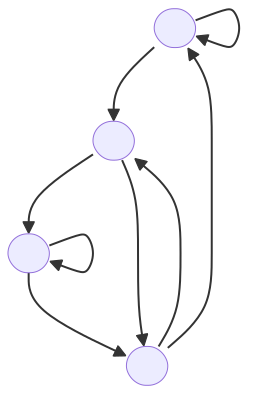
\includegraphics[width=0.5\linewidth]{./img/fuente-de-markov-diagrama-de-estados.png}
\end{figure}

\begin{center}\rule{0.5\linewidth}{0.5pt}\end{center}

Se dice que una fuente de Markov es ergódica si es posible pasar de
cualquier estado a cualquier otro estado en un número finito de pasos.

\begin{center}\rule{0.5\linewidth}{0.5pt}\end{center}

\paragraph{Ejemplo}\label{ejemplo}

Una fuente ergódica podría ser la anterior (podemos alcanzar cualquier
estado en un número finito de pasos a partir de otro estado).

Ejemplo de diagrama de estados de una fuente ergódica:

\begin{figure}[htbp!]
\centering
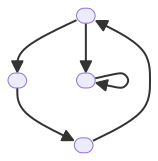
\includegraphics[width=0.25\linewidth]{./img/fuente-de-markov-no-ergódico.png}
\end{figure}

Nótese que el nodo interior es un estado absorbente. Es decir, una vez
que se llega a ese estado, no se puede salir de él.

\begin{center}\rule{0.5\linewidth}{0.5pt}\end{center}

Una fuente de Markov es homogénea si las probabilidades condicionales no
cambian con el tiempo.

Se dice que una fuente está en estado estacionario si la probabilidad de
observación de sus estados no cambia con el tiempo. Las probabilidades
se pueden obtener mediante la ecuación \(v=\pi\Pi\), donde \(\pi\) es el
vector de probabilidad de los estados y \(\Pi\) es la matriz de
transición.

\begin{center}\rule{0.5\linewidth}{0.5pt}\end{center}

\paragraph{Ejemplo}\label{ejemplo-1}

Volviendo al ejemplo inicial, la matriz de probabilidades tiene la
siguiente forma:

\[
\Pi = \begin{matrix}
& \begin{matrix} 00 & 01 & 10 & 11 \end{matrix} \\
\begin{matrix} 00 \\ 01 \\ 10 \\ 11 \end{matrix} & \begin{pmatrix} 0.7 & 0.5 & 0.5 & 0.3 \\ 0.5 & 0.5 & 0.5 & 0.5 \\ 0.5 & 0.5 & 0.5 & 0.5 \\ 0.3 & 0.5 & 0.5 & 0.7 \end{pmatrix}
\end{matrix}
\]

Véase que cada fila suma 1 (debido a los axiomas de Kolmogorov). Si cada
columna sumase 1, entonces la matriz es doblemente estocástica y todos
los estados son equiprobables.

Vayamos al cálculo de probabilidades de estados en régimen estacionario.
Para ello, nos definimos las siguientes ecuaciones:


\begin{align*}
&P(00) = P(0|00)\cdot P(00) + P(0|10)\cdot P(10)\\
&P(01) = P(1|00)\cdot P(00) + P(0|10)\cdot P(10)\\
&P(11) = P(1|01)\cdot P(01) + P(1|11)\cdot P(11)\\
&P(00) + P(01) + P(10) + P(11) = 1
\end{align*}


Nótese que la última ecuación surge por uno de los axiomas de
Kolmogorov, ya que si incluyésemos el estado \(01\) en la primera
ecuación, tendríamos una ecuación redundante (y por ende un sistema
singular; con infinitas soluciones). Conocemos las probabilidades
condicionaes, por lo que podemos resolver el sistema de ecuaciones:


\begin{align*}
&P(00) = 0.7\cdot P(00) + 0.5\cdot P(10)\\
&P(01) = 0.3\cdot P(00) + 0.5\cdot P(10)\\
&P(11) = 0.5\cdot P(01) + 0.7\cdot P(11)\\
&P(00) + P(01) + P(10) + P(11) = 1
\end{align*}


Este sistema tiene la siguiente solución:

\[
\pi = \begin{pmatrix} P(00) \\ P(01) \\ P(10) \\ P(11) \end{pmatrix} = \begin{pmatrix} \frac{5}{16} \\ \frac{3}{16} \\ \frac{3}{16} \\ \frac{5}{16} \end{pmatrix}
\]

Ahora, con esta información podemos calcular las probabilidades de
aparición de cada símbolo:


\begin{align*}
&P(0) = P(00) + P(10) = \frac{5}{16} + \frac{3}{16} = \frac{8}{16} = \frac{1}{2}\\
&P(1) = P(01) + P(11) = \frac{3}{16} + \frac{5}{16} = \frac{8}{16} = \frac{1}{2}
\end{align*}


\begin{center}\rule{0.5\linewidth}{0.5pt}\end{center}

\subsubsection{Fuentes afines (adjuntas) de una fuente de
Markov}\label{fuentes-afines-adjuntas-de-una-fuente-de-markov}

Dada una fuente de Markov de orden \(m\) con un alfabeto \(\mathcal{S}\)
y una distribución de probabilidad \(P\), denominaremos a la fuente afín
como a la fuente de memoria nula \((\mathcal{S},P)\). Es decir, la
fuente afín es la fuente de memoria nula que emite los mismos símbolos
que la fuente de Markov.

\begin{center}\rule{0.5\linewidth}{0.5pt}\end{center}

\paragraph{Ejemplo}\label{ejemplo-2}

Para el ejemplo de la fuente de Markov de orden 2, la fuente afín sería
la fuente de memoria nula con \(\mathcal{S}=\left\{0,1\right\}\) y
\(P=\left\{\frac{1}{2},\frac{1}{2}\right\}\).

\begin{center}\rule{0.5\linewidth}{0.5pt}\end{center}

Para el cálculo de entropía de una fuente de Markov de orden \(m\),
sobre un alfabeto \(\mathcal{S}=\left\{s_1,s_2,\dots,s_n\right\}\) y
distribución de probabilidad condicional
\(P(s_i|s_{i_1},\dots,s_{i_m})\), se cumple que
\(p(s_i, s_{i_1},\dots,s_{i_m}) = p(s_i|s_{i_1},\dots,s_{i_m})\cdot p(s_{i_1},\dots,s_{i_m})\),
lo cual nos permite calcular la entropía condicional:

\[
H(\mathcal{S}|s_{i_1},\dots,s_{i_m}) = -\sum_{i=1}^{n}p(s_i|s_{i_1},\dots,s_{i_m})\log\left(p(s_i|s_{i_1},\dots,s_{i_m})\right)
\]

Por lo tanto, la entropía de la fuente de Markov de orden \(m\) es:


\begin{align*}
H(\mathcal{S}) &= \sum_{\mathcal{S}^m}p(s_{i_1},\dots,s_{i_m})H(\mathcal{S}|s_{i_1},\dots,s_{i_m})\\
&= -\sum_{\mathcal{S}^m}p(s_{i_1},\dots,s_{i_m})\left(-\sum_{s_i\in\mathcal{S}}p(s_i|s_{i_1},\dots,s_{i_m})\log\left(p(s_i|s_{i_1},\dots,s_{i_m})\right)\right)\\
&= -\sum_{\mathcal{S}^{m+1}}p(s_i, s_{i_1},\dots,s_{i_m})p(s_i|s_{i_1},\dots,s_{i_m})\log\left(p(s_i|s_{i_1},\dots,s_{i_m})\right)\\
&= -\sum_{\mathcal{S}^{m+1}}p(s_{i_1},\dots,s_{i_m},s_i)\log\left(p(s_i|s_{i_1},\dots,s_{i_m})\right)\\
\end{align*}



\subsection{Códigos}\label{cuxf3digos}

\subsubsection{Introducción}\label{introducciuxf3n-codigos}

Como hemos visto al principio del temario, existe un componente en el
esquema de transmisión de información llamado \textbf{codificador}, el
cual se encarga de transformar los mensajes de la fuente (\texttt{MF})
en una forma adecuada para su transmisión a través del canal de
comunicación y recepción (mensajes codificados, \texttt{MC}), donde se
lleva a cabo el proceso correspondiente de decodificación para la
recuperación del mensaje fuente original \texttt{MF}.

En una primera aproximación simplificada a este escenario, definimos el
proceso de codificación mediante una función \(f\) tal que

\[
f:\text{\texttt{MF}}\rightarrow\mathcal{P}(\text{\texttt{MC}})
\]

donde \(\forall m\in\text{\texttt{MC}}: \left|f(m)\right|<\infty\) (es
decir que los resultados de la codificación del mensaje tienen una
longitud finita). Nótese que \(\mathcal{P}(C)\) significa el conjunto
potencia de \(C\).

Por lo tanto, en este contexto de transmisión de información, cuando se
emite un mensaje aletorio \(m\), el receptor recibe un mensaje
codificado \(m'\in\mathcal{P}(C)\). Entonces, existe en el receptor una
función \(f^\star\) de decodificación:

\[
f^\star:\text{\texttt{MC}}\rightarrow\text{\texttt{MF}}
\]

tal que

\[
\forall m\in \text{\texttt{MF}}, \quad\exists m': f^\star\left(m'\right) = m
\]

Por ahora asumiremos que
\(\forall m\in \text{\texttt{MF}}, \left|f(m)\right| = 1\) (pero veremos
que nos podremos extender a más casos).

\subsubsection{Codificaciones y
códigos}\label{codificaciones-y-cuxf3digos}

Llevando la introducción anterior a un caso más particular (y familiar);
sea \(\mathcal{A}\) un alfabeto (correspondiente a la fuente de
información de memoria nula \((\mathcal{A},P)\), de la que se originan
los mensajes fuente \(\mathcal{A^+}\)) y sea \(\mathcal{C}\) el conjunto
de los mensajes codificados \texttt{MC} (también conocido como el
conjunto de códigos), entonces una codificación \(f\) es una aplicación
\textbf{biyectiva}:

\[
f:\mathcal{A}^+\rightarrow\mathcal{C}
\]

Para que esta codificación sea admisible para un proceso eficiente de
codificación-decodificación, deberá tener unas características
determinadas que se irán exponiendo más adelante.

Sea \(\mathcal{B}\) un alfabeto (código), entonces
\(\mathcal{C}\subseteq\mathcal{B}\). Entonces una codificación admisible
es una aplicación inyectiva

\[
f:\mathcal{A}^+\rightarrow\mathcal{B}^+
\]

en la que tenemos que \(f\left(\mathcal{A}^+\right) = \mathcal{C}\).
Equivalentemente, si tomamos \(f(\lambda) = \lambda\) (y también
\(f^-1(\lambda) = \left\{\lambda\right\}\)), entonces podemos extender
esta aplicación inyectiva a

\[
f:\mathcal{A}^*\rightarrow\mathcal{B}^*
\]

En este escenario \(\mathcal{A}\) recibe el nombre de ``\emph{alfabeto
fuente}'' y \(\mathcal{B}\) ``\emph{alfabeto código}''.

\subsubsection{Codificación Bloque}\label{codificaciuxf3n-bloque}

Una codificación bloque \(f\) es una aplicación que le asigna a cada uno
de los símbolos \(a\in\mathcal{A}\) una palabra de \(\mathcal{B}^+\), y
se comporta como un homomorfismo, lo cual quiere decir que

\[
\forall x\in\mathcal{A}^+,\forall a\in\mathcal{A}: f(ax) = f(a)f(x)
\]

y de forma equivalente

\[
\forall x\in\mathcal{A}^+,\forall a\in\mathcal{A}: f(xa) = f(x)f(a)
\]

y de forma general

\[
\forall x,y\in\mathcal{A}^+: f(xy) = f(x)f(y)
\]

Por tanto

\[
\forall x\in\mathcal{A}^+: f(x) = f(x[1])\dots f(x[|x|])
\]

\emph{(todo esto es equivalente, y lo hemos visto anteriormente en la
definición de homomorfismo en el apartado de estructura del lenguage)}

El conjunto
\(f(\mathcal{A})=\left\{f(a),\quad\forall\mathcal{A}\right\}\) recibe el
nombre de ``\emph{código bloque}'' (o simplemente ``\emph{código}'').

\paragraph{Ejemplo 1}\label{ejemplo-1-codigos}

Consideremos los siguientes alfabetos fuente (\(\mathcal{A}\)) y código
(\(\mathcal{B}\)):


\begin{align*}
\mathcal{A} &=\left\{0,1,2,3,4,5,6,7,8,9\right\}\\
\mathcal{B} &=\left\{0,1\right\}
\end{align*}


y además consideremos la codificación de bloque definida por \(f\):

\[
f(a) = \left(\left\lfloor\frac{a_1}{2^0}\right\rfloor\right)\left(\left\lfloor\frac{a_2}{2^1}\right\rfloor\right)\left(\left\lfloor\frac{a_3}{2^2}\right\rfloor\right)\left(\left\lfloor\frac{a_4}{2^3}\right\rfloor\right)
\]

claramente tenemos que

\[
f(\mathcal{A}) = \left\{0000, 0001, 0010, 0011, 0100, 0101, 0110, 0111, 1000, 1001\right\}
\]

Se puede ver que \(f(\mathcal{A})\subset\mathcal{B}^4\) (porque hay
palabras en \(\mathcal{B}^4\) que no aparecen en \(f(\mathcal{A})\),
como por ejemplo \(1111\)). \(f\) es una codificación de bloque ya que
le asigna a cada caracter del alfabeto fuente, una palabra formada por
el alfabeto código.

\paragraph{Ejemplo 2: Morse}\label{ejemplo-2-morse}

En el morse, el alfabeto código consta de los elementos
\(\left\{\cdot,-,\text{\texttt{pausa}}\right\}\):

\begin{longtable}[]{@{}ll@{}}
\toprule\noalign{}
Alfabeto fuente & Código \\
\midrule\noalign{}
\endhead
\bottomrule\noalign{}
\endlastfoot
A & .- \\
B & -\ldots{} \\
C & -.-. \\
D & -.. \\
E & . \\
F & ..-. \\
G & --. \\
H & \ldots. \\
I & .. \\
J & .--- \\
K & -.- \\
L & .-.. \\
M & -- \\
N & -. \\
P & .--. \\
Q & --- \\
S & \ldots{} \\
T & - \\
U & ..- \\
V & \ldots- \\
W & .-- \\
X & -..- \\
Y & -.-- \\
Z & --.. \\
1 & .---- \\
2 & ..--- \\
3 & \ldots-- \\
4 & \ldots.- \\
5 & \ldots.. \\
6 & -\ldots. \\
7 & --\ldots{} \\
8 & ---.. \\
9 & ----. \\
0 & ---- \\
\end{longtable}

Al codificar un mensaje en morse, después del código asociado a cada
simbolo ha de introducirse una pausa de separación.

\paragraph{Ejemplo 3: ASCII}\label{ejemplo-3-ascii}

El ASCII (\emph{American Standard Code for Information Interchange}) es
una codificación bloque de logitud constante (no como el morse, que era
de longitud variable) con alfabeto código
\(\mathcal{B}=\left\{0,1\right\}\) y
\(f(\mathcal{A})=\left\{0,1\right\}^7\).

\paragraph{Ejemplo 4: ASCII Extendido}\label{ejemplo-4-ascii-extendido}

El ASCII extendido es diferencia del ASCII por
\(f(\mathcal{A})=\left\{0,1\right\}^8\) (la longitud de las palabras es
mayor).

\paragraph{Unicode}\label{unicode}

Unicode es un alfabeto universal junto con la codificación de sus
símbolos (más de un millón) mediante un código bloque de longitud fija e
incorpora todos los símbolos del ASCII extendido. A partir de Unicode se
encuentran, entre otras, las codificaciones bloques de longitud variable
UTF (Unicode Transformation Format): UTF-8 (la más común), UTF-16 y
UTF-32.

\subsubsection{Codificación Bloque Unívocamente
Decodificable}\label{codificaciuxf3n-bloque-unuxedvocamente-decodificable}

Una codificación de bloque \(f\) se llama \textbf{no singular} siempre
que

\[
\forall a,b\in\mathcal{A}: a\neq b\Rightarrow f(a)\neq f(b)
\]

\paragraph{Ejemplo 1}\label{ejemplo-1-1-codigos}

Sea \(\mathcal{A} = \left\{a_1,a_2,a_3,a_4\right\}\), \(\mathcal{B} =
\left\{0,1\right\}\) y \(f\) definida por:

\[
f = \begin{cases}
f(a_1) &= 0\\
f(a_2) &= 11\\
f(a_3) &= 00\\
f(a_4) &= 01\\
\end{cases}
\]

Es sencilo ver que \(f\) es no singular. Sin embargo, si nos extendemos
a palabras, esto ya no se cumple ya que ciertas palabras de
\(\mathcal{A}^+\) no son unívocamente decodificables. Por ejemplo:

\begin{itemize}
\tightlist
\item
  \(a_1a_1a_1\neq a_1a_3\neq a_3a_1\) pero
  \(000 = f(a_1a_1a_1 ) = f(a_1a_3) = f(a_3a_1)\)
\item
  \(a_1a_1a_2\neq a_3a_2\) pero \(0011 = f(a_1a_1a_2) = f(a_3a_2)\)
\end{itemize}

\begin{center}\rule{0.5\linewidth}{0.5pt}\end{center}

La extensión de orden \(n\geq 1\)de una codificación bloque

\[
f:\mathcal{A}^+\rightarrow\mathcal{B}^+
\]

se define como

\[
f^{(n)}:\left(\mathcal{A}^n\right)^+\rightarrow\mathcal{B}^+
\]

tomando como símbolos las palabras de \(\mathcal{A}^n\) de forma que

\[
\forall x\in\mathcal{A}^n: f^{(n)}(x)=f(x)
\]

La extensión de orden \(n\) de una codificación bloque también lo es
tomando, para cada caso, como alfabeto fuente el correspondiente
\(\mathcal{A}\).

Una codificación bloque \(f\) se dice unívocamente decodificable sí y
sólo si su extensión de orden \(n\) es \textbf{no singular} para cada
\(n\geq 1\).

Surge una propiedad importante: una codificación bloque es unívocamente
decodificable si y sólo si es inyectiva.

Diremos que un código bloque es unívocamente decodificable si proviene
de una codificación bloque unívocamente decodificable, lo cual nos
permite definir \(f^{-1}:\mathcal{B}^+\rightarrow\mathcal{A}^+\).

\textbf{Propiedad de factorización única:}

\begin{enumerate}
\def\labelenumi{\arabic{enumi}.}
\tightlist
\item
  Si \(f:\mathcal{A}^+\rightarrow\mathcal{B}^+\) es una codificación
  bloque unívocamente decodificable, entonces se tiene que
  \(\forall x_1,\dots,x_n,y_1,\dots,y_m\in f(\mathcal{A})\):
\end{enumerate}

\[
x_1\dots x_n=y_1\dots y_m \Rightarrow (n = m)\wedge\left(x_i=y_i,\quad i = 1,\dots,n\right)
\]

\begin{enumerate}
\def\labelenumi{\arabic{enumi}.}
\setcounter{enumi}{1}
\tightlist
\item
  \(f:\mathcal{A}^+\rightarrow\mathcal{B}^+\) (que es una codificación
  bloque) es unívocamente decodificable si y solamente si cumple la
  propiedad mencionada anteriormente, y además es no singular.
\end{enumerate}

La cuestión de si una codificación bloque \(f\) es unívocamente
decodificable o no es algorítmicamente decidible (\emph{es decir, que
hay un algoritmo para averiguar si es unívocamente decodificable o no}).

El siguiente algoritmo devuelve \texttt{true} cuando \(f\) es
unívocamente decodificable y \texttt{false} en caso contrario:


\begin{align*}
&\text{if }\left(\exists a,b\in\mathcal{A}: (a\neq b)\wedge(f(a)=f(b))\right)\text{then:}\\
&\quad\quad\text{return \texttt{false}}\\
&A=\left\{u: \left(\exists x,y\in f(\mathcal{A}):(x\neq y)\wedge (xu=y)\right)\right\}\\
&\text{if}\left(A\cap f(A)\neq\emptyset\right)\text{ then:}\\
&\quad\quad\text{return \texttt{false}}\\
&A'=\emptyset\\
&\text{while }A'\neq\emptyset:\\
&\quad\quad A'=A\cup A'\\
&\quad\quad B = \left\{u:\left(\left(\exists x\in f(\mathcal{A}): xu\in A\right)\vee\left(\exists x\in A: xu\in f(\mathcal{A})\right)\right)\right\}\\
&\quad\quad A = B - A'\\
&\quad\quad\text{if }\left(A\cap f(\mathcal{A})\neq\emptyset\right)\text{ then:}\\
&\quad\quad\quad\quad\text{return \texttt{false}}\\
&\text{return \texttt{true}}\\
\end{align*}


Sea \(f:\mathcal{A}^+\rightarrow\mathcal{B}^+\) una codificación bloque
no singular. Si todas las palabras del código bloque tienen exactamente
la misma longitud, entonces el código es unívocamente decodificable.

\emph{Piensa en el Ejemplo 1 de esta sección. ¿De dónde salían los
problemas a la hora de decodificar? Surgían del hecho de que no todas
lass palabras del código bloque tenían la misma longitud}

\subsubsection{Desigualdad de McMillan}\label{desigualdad-de-mcmillan}

Si \(f:\mathcal{A}^+\rightarrow\mathcal{B}^+\) es una codificación
bloque unívocamente decodificable y \(\left|\mathcal{B}\right|=k\),
entonces

\[
\sum_{x\in f(\mathcal{A})} k^{-\left|x\right|}\leq 1
\]

\paragraph{Ejemplo 1}\label{ejemplo-1-2}

Recuperando el ejemplo anterior de los siguientes alfabetos fuente
(\(\mathcal{A}\)) y código (\(\mathcal{B}\)):


\begin{align*}
\mathcal{A} &=\left\{0,1,2,3,4,5,6,7,8,9\right\}\\
\mathcal{B} &=\left\{0,1\right\}
\end{align*}


con

\[
f(\mathcal{A}) = \left\{0000, 0001, 0010, 0011, 0100, 0101, 0110, 0111, 1000, 1001\right\}
\]

La desigualdad de McMillan debería de cumplirse ya que es una
codificación bloque unívocamente decodificable:

\[
\sum_{x\in f(\mathcal{A})} k^{-\left|x\right|} = \sum_{x\in f(\mathcal{A})} 2^{-4} = \frac{10}{16} < 1
\]

Vemos rápidamente que se cumple.

\emph{¿Qué condición debería cumplirse para tener la igualdad estricta?}

Imaginémonos ahora que tenemos


\begin{align*}
\mathcal{A} &=\left\{0,1,2,3,4,5,6,7,8,9,a,b,c,d,e,f\right\}\\
\mathcal{B} &=\left\{0,1\right\}
\end{align*}


con

\[
f(\mathcal{A}) = \left\{0000, 0001, 0010, 0011, 0100, 0101, 0110, 0111, 1000, 1001,1010,1011,1100,1101, 1110,1111\right\}
\]

\emph{(¿no resulta esto familiar? Es la representación en binario del
hexadecimal)}

Para este caso:

\[
\sum_{x\in f(\mathcal{A})} k^{-\left|x\right|} = \sum_{x\in f(\mathcal{A})} 2^{-4} = \frac{16}{16} = 1
\]

Claramente cuando \(f(\mathcal{A})\subset\mathcal{B}^+\), entonces la
desigualdad es estricta. Pero cuando \(f(\mathcal{A})=\mathcal{B}^+\),
entonces tenemos la igualdad.

\subsubsection{Códigos instantáneos}\label{cuxf3digos-instantuxe1neos}

Empecemos observando un ejemplo. Consideremos la codificación
unívocamente decodificable \(f(a)=0\) y \(f(b)=01\). Para decodificar
\(x=01\), tendríamos que conocer de la existencia del \(1\), ya que
únicamente con el \(0\) tenemos una ambigüedad y no sabemos si se trata
de \(a\) o de \(b\). Al leer el \(1\), resolvemos esto y podemos
decodificar \(x\) como \(b\). Es decir, hasta no leer la palabra entera,
no hemos podido saber cómo decodificarla.

Esta situación empeora cuanto más larga es la palabra, y puede llevar a
que la decodificación sea impracticable.

Consideremos ahora la codificación unívocamente decodificable
\(f(a)=0\), \(f(b)=01\) y \(f(c)=11\). Sea \(x=01^n\) con \(n\geq 1\).
Tenemos que

\[
f^-1(x) = \begin{cases}
ac^m&\quad\text{si }n\text{ es par, con }m=\frac{n}{2}\\
bc^m&\quad\text{si }n\text{ es impar, con }m=\frac{n-1}{2}
\end{cases}
\]

Veamos una serie de ejemplos:

\begin{itemize}
\tightlist
\item
  \(f^-1(x)=f^-1(01^6)=f^-1(0111111)=accc\)
\item
  \(f^-1(x)=f^-1(01^{11})=f^-1(011111111111)=bccccc\)
\end{itemize}

Para decodificar, es esencial conocer cuantos \(1\) tenemos en la
palabra \(x\). Esto no lo podemos averiguar si no leemos toda la palabra
primero (independientemente de lo larga que sea esta), antes de
decodificar.

Se dice que un código unívocamente decodificable es \textbf{instantáneo}
cuando es posible decodificar cada símbolo de \(\mathcal{A}\) de cada
mensaje sin necesitar más símbolos de \(\mathcal{B}\) de los
estricamente necesarios. Es decir, si

\[
h:\mathcal{A}^*\rightarrow\mathcal{B}^*
\]

es una codificación bloque unívocamente decodificable, entonces es
instantánea siempre que

\[
\forall x\in\mathcal{A}^*, \exists u,v\in\mathcal{A}^*,\exists a\in\mathcal{A}: x=uav
\]

tal que

\[
y=h(x)=h(u)h(a)h(v)
\]

Entonces para decodificar \(y\) a \(x\), para decodificar el segmento
\(h(a)\) a \(a\) de forma inmediata, independientemente del sufijo
\(h(v)\), solamente hay que procesar el segmento de \(y\) asociado a
\(h(a)\).

Entonces para descodificar el segmento
\(y\left[\left|h(u)\right|+1:\left|h(u)\right|+n\right]\) con, en este
caso, \(n = \left|h(a)\right|\):


\begin{align*}
y\left[\left|h(u)\right|+1:\left|h(u)\right|+n\right] &= y\left[\left|h(u)\right|+1:\left|h(u)\right|+\left|h(a)\right|\right]\\
&= y\left[\left|h(u)\right|+1:\left|h(ua)\right|\right]
\end{align*}


es suficiente, en cualquier caso, para la correcta decodificación. Eso
quiere decir que

\[
\forall a,b\in\mathcal{A}:h(a)\text{ es prefijo de }h(b)\Rightarrow a = b
\]

Una vez más, diremos que un código bloque es instantáneo cuando proviene
de una codificación bloque instantánea. También podemos llamarlo código
bloque prefijo o simplemente código prefijo.

\begin{center}\rule{0.5\linewidth}{0.5pt}\end{center}

Sea \(f:\mathcal{A}^*\rightarrow\mathcal{B}^*\) una codificación de
bloque. Diremos que \(f\) es \textbf{estable} siempre que:

\begin{enumerate}
\def\labelenumi{\arabic{enumi}.}
\tightlist
\item
  Sea unívocamente decodificable.
\item
  \(\forall x\in\mathcal{A}^*,f(x)=u\) se cumple que
  \(\forall v\in\mathcal{B}^*\), si
  \(\exists y\in\mathcal{A}^*,f(y)=uv\Rightarrow y=xz\) para algún
  \(z\in\mathcal{A}^*\)
\end{enumerate}

Tenemos entonces la siguiente propiedad: sea
\(f:\mathcal{A}^*\rightarrow\mathcal{B}^*\) una codificación bloque.
Entonces, \textbf{\(f\) es estable si y sólo si es instantánea}.

\begin{center}\rule{0.5\linewidth}{0.5pt}\end{center}

\subsubsection{Desigualdad de Kraft}\label{desigualdad-de-kraft}

Veamos cómo estad características cualitativas se traducen
cuantitativamente. Sea la codificación bloque:

\[
f:\mathcal{A}^*\rightarrow\mathcal{B}^*
\]

con \(\mathcal{A}=\left\{a_1,\dots,a_n\right\}\),
\(\mathcal{B}=\left\{b_1,\dots,b_k\right\}\) y
\(f\left(\mathcal{A}\right)=\left\{x_1,\dots,x_n\right\}\), con
\(l_i = \left|x_i\right|\). La desigualdad de Kraft nos da la condición
\textbf{necesaria} y \textbf{suficiente} para que exista un código
bloque isntantáneo con palabras de su código bloque de longitud
\(l_1,\dots,l_n\) sobre un alfabeto con \(k\) símbolos:

\[
\sum_{1\leq i\leq n}k^{l_i}\leq 1
\]

Cuando esto es una igualdad estricta, se conoce como la igualdad de
Kraft.

Como consecuencia inmediata, a partir de la desigualdad de McMillan, se
tiene que para cada código unívocamente decodificable se tiene un código
instantáneo con las mismas longitudes de las palabras de su código
bloque.

\subsubsection{Códigos Completos}\label{cuxf3digos-completos}

Sea la codificación de bloque:

\[
f:\mathcal{A}^*\rightarrow\mathcal{B}^*
\]

diremos que es completa si:ç

\begin{enumerate}
\def\labelenumi{\arabic{enumi}.}
\tightlist
\item
  Es instantánea.
\item
  Cumple que
  \(\forall x\in\mathcal{B}^*,\exists a\in\mathcal{A}^*\Rightarrow\left(\left(h(a)\text{ es prefijo de }x\right)\vee\left(x\text{ es prefijo de }h(a)\right)\right)\).
\end{enumerate}

Tenemos entonces la siguiente propiedad: si
\(\left|\mathcal{A}\right|\geq 2\) y \(\left|\mathcal{B}\right|=2\),
entonces sólo existe una codificación de bloque completa

\[
f':\mathcal{A}^*\rightarrow\mathcal{B}^*
\]

tal que
\(\forall a\in\mathcal{A}:\left|f'(a)\right|\leq\left|f(a)\right|\).

Nuevamente, un código bloque es completo si proviene de una codificación
de bloque completa.

\subsection{Codificaciones de Fuentes de
Información}\label{codificaciones-de-fuentes-de-informaciuxf3n}

\subsubsection{Longitud media de un
código}\label{longitud-media-de-un-cuxf3digo}

Para un \(\mathcal{A}^*\) y \(\mathcal{B}^*\), es posible definir más de
una codificación instantánea o unívocamente decodificable. Esto requiere
entonces que intentemos elegir las más eficientes con el objetivo de
tener una transmisión de información óptima.

Un criterio natural de selección (aún cuando no es el único posible) es
el de la mínima longitud media.

Sea un código bloque que asocia los símbolos de una \textbf{fuente de
información de memoria nula} \(FI = \left(\mathcal{A},P\right)\) donde
\(\mathcal{A}=\left\{a_1,\dots,a_n\right\}\) y
\(\left|\mathcal{B}\right|=k\) mediante la codificación
\(f:\mathcal{A}^*\rightarrow\mathcal{B}^*\) con las palabras
\(f\left(a_i\right)=x_i\), con \(l_i=\left|x_i\right|,i=1,\dots,n\).
Definimos la lonfitud media como la \textbf{esperanza matemática de la
longitud de los códigos bloque}:

\[
\mathcal{L}_f=\mathbb{E}\left[l\right]=\mathbb{E}\left[\left|x\right|\right]=\mathbb{E}\left[\left|f(a)\right|\right]=\sum_{i=1}^n \left|f(a_i)\right|p(a_i)
\]

\subsubsection{Códigos óptimos}\label{cuxf3digos-uxf3ptimos}

Sea un código bloque unívocamente decodificable que asocia los símbolos
de la fuente de memoria nula \(FI = \left(\mathcal{A},P\right)\) con
palabras formadas por un alfabeto \(\left|\mathcal{B}\right|=k\).
Diremos que es \textbf{compacto} u \textbf{óptimo} con respecto a la
fuente de información si su longitud media es menor o igual que la
longitud media de cada uno de los códigos bloque unívocamente
decodificables que pueden definirse entre la fuente y alfabetos códigos
con \(k\) símbolos.

Surge de aquí la observación de que, puesto que esto incide únicamente
sobre las logitudes, la búsqueda puede reducirse por la desigualdad de
McMillan a códigos instantáneos.

Además, si se tiene que \(\left|\mathcal{A}\right|\geq 2\) y
\(\left|\mathcal{B}\right| = 2\), si un código bloque es óptimo,
entonces es completo.

También se tiene la propiedad de si \(f\) es un código óptimo, entonces

\[
\forall a,b\in\mathcal{A}:p(a)<p(b)\Rightarrow \left|f(a)\right|\geq\left|f(b)\right|
\]

\subsubsection{\texorpdfstring{Primer Teorema de Shannon \emph{(teorema
de la codificación sin
ruido)}}{Primer Teorema de Shannon (teorema de la codificación sin ruido)}}\label{primer-teorema-de-shannon-teorema-de-la-codificaciuxf3n-sin-ruido}

Consideremos una fuente de memoria nula \(FI\) cuyos símbolos
\(a_1,\dots,a_n\) con probabilidades \(p_1,\dots,p_n\) se codifican cada
uno en una palabra de longitud \(l_i\) en un alfabeto con \(k\) símbolos
mediante la codificación \(f\). Entonces se tiene que
\(H_k\left(FI\right)\leq\mathcal{L}_f\).

Si suponemos que nos encontramos en el caso de la igualdad, es decir,
\(H_k\left(FI\right)=\mathcal{L}_f\):


\begin{align*}
H_k\left(FI\right)&=\mathcal{L}_f\\
\sum_{i=1}^np_i\log_k\left(\frac{1}{p_i}\right)&=\sum_{i=1}^np_il_i
\end{align*}


inferimos que si tomamos longitudes de código
\(l_i=\left|x_i\right|=\left|f(a_i)\right|\), tendremos que los códigos
obtenidos para cada \(a_i\) serán instantáneos, completos y óptimos con
una longitud media que coincide con la entropía en base \(k\) de la
fuente de información (asumiendo claramente que
\(\log_k\left(\frac{1}{p_i}\right)\) es un número entero
\(\forall 1\leq i\leq n\)).

Veamos un ejemplo: supón que tenemos
\(FI=\left(\left\{a_1,a_2,a_3\right\},\left\{\frac{1}{2},\frac{1}{4},\frac{1}{4}\right\}\right)\),
entonces la codificación de bloque:

\[
h:\left\{a_1,a_2,a_3\right\}^*\rightarrow\left\{0,1\right\}^*
\]

definida tomando las longitudes de los códigos como
\(\log\left(\frac{1}{p_i}\right)\):

\[
h=\begin{cases}
h\left(a_1\right) &= 1\\
h\left(a_2\right) &= 00\\
h\left(a_3\right) &= 01
\end{cases}
\]

es instantánea, completa y óptima con
\(\mathcal{L}_h=H\left(FI\right)\).

Pero, ¿qué sucede si resulta que \(\log_k\left(\frac{1}{p_i}\right)\) no
resultan ser números enteros? Parece intuitivo y apropiado en este
contexto redondear el valor obtenido hacia arriba, para elegir \(l_i\)
(aunque claramente en este caso, el código obtenido no tiene por qué ser
optimo). Entonces si
\(l_i=\left\lceil\log_k\left(\frac{1}{p_i}\right)\right\rceil\), por
definición se tiene que

\[
\log_k\left(\frac{1}{p_i}\right)\leq l_i\leq\log_k\left(\frac{1}{p_i}\right) + 1
\]

Se puede demostrar que se cumple la desigualdad de Kraft. Tomemos
\(\log_k\left(\frac{1}{p_i}\right)\leq l_i\):


\begin{align*}
\log_k\left(\frac{1}{p_i}\right)&\leq l_i\\
k^{\log_k\left(\frac{1}{p_i}\right)}&\leq k^{l_i}\\
\frac{1}{p_i}&\leq k^{l_i}\\
\frac{1}{k^{l_i}}&\leq p_i\\
k^{-l_i}&\leq p_i,\quad\forall 1\leq i\leq n\\
\sum_{i=1}^nk^{-l_i}&\leq\sum_{i=1}^n p_i\\
\sum_{i=1}^nk^{-l_i}&\leq 1
\end{align*}


En consecuencia, pueden asociárseles códigos bloque instantáneos.

Volviendo a la siguiente desigualdad:

\[
\log_k\left(\frac{1}{p_i}\right)\leq l_i\leq\log_k\left(\frac{1}{p_i}\right) + 1
\]

Multiplicando todos los términos por \(p_i\):

\[
p_i\log_k\left(\frac{1}{p_i}\right)\leq p_il_i\leq p_i\log_k\left(\frac{1}{p_i}\right) + p_i
\]

y sumando ya que la desigualdad se cumple \(\forall 1\leq i\leq n\):


\begin{align*}
\sum_{i=1}^np_i\log_k\left(\frac{1}{p_i}\right)&\leq\sum_{i=1}^np_il_i\leq \sum_{i=1}^np_i\log_k\left(\frac{1}{p_i}\right) + \sum_{i=1}^np_i\\
H_k\left(FI\right)&\leq\mathcal{L}_f\leq H_k\left(FI\right) + \sum_{i=1}^np_i\\
H_k\left(FI\right)&\leq\mathcal{L}_f\leq H_k\left(FI\right) + 1\\
\end{align*}


Cumpliéndose esto también para cualquier código óptimo, lo que
constituye la formulación inicial del primer teorema de Shannon.

Puesto que esto puede aplicarse además a cualquier extensión de grado
\(m\) de una fuente de memoria nula\ldots{}


\begin{align*}
H_k\left(FI^{(m)}\right)&\leq\mathcal{L}_f^m\leq H_k\left(FI^{(m)}\right) + 1\\
mH_k\left(FI\right)&\leq\mathcal{L}_f^m\leq mH_k\left(FI\right) + 1\\
H_k\left(FI\right)&\leq\frac{\mathcal{L}_f^m}{m}\leq H_k\left(FI\right) + \frac{1}{m}\\
\end{align*}


Obteniendo así \textbf{el primer teorema de Shannon}, que es uno de los
teoremas fundamentales de la teoría de la información.

Una propiedad interesante surge cuando intentamos ver qué pasa cuando la
extensión de grado \(m\) de nuestra fuente de información de memoria
nula emite palabras largas. Para ello tenemos que ver qué sucede cuando
\(m\to\infty\):


\begin{align*}
\lim_{m\to\infty}H_k\left(FI\right)&\leq\lim_{m\to\infty}\frac{\mathcal{L}_f^m}{m}\leq \lim_{m\to\infty}H_k\left(FI\right) + \lim_{m\to\infty}\frac{1}{m}\\
H_k\left(FI\right)&\leq\lim_{m\to\infty}\frac{\mathcal{L}_f^m}{m}\leq H_k\left(FI\right) + 0\\
\end{align*}


Como \(\lim_{m\to\infty}\frac{\mathcal{L}_f^m}{m}\) queda acotado por
arriba y por abajo por \(H_k\left(FI\right)\), hemos demostrado mediante
``\emph{el teorema del sándwich}'' que

\[
\lim_{m\to\infty}\frac{\mathcal{L}_f^m}{m} = H_k\left(FI\right)
\]

Nótese que \(\frac{\mathcal{L}_f^m}{m}\) es el \textbf{número medio de
símbolos del alfabeto código (\(\mathcal{B}\)) empleados en la
codificación de un símbolo del alfabeto fuente (\(\mathcal{A}\)) cuando
se emiten secuencias de longitud \(m\), es decir, como símbolos del
alfabeto \(\mathcal{A}^{(m)}\)}.

\begin{center}\rule{0.5\linewidth}{0.5pt}\end{center}

\paragraph{Ejemplo Aplicado}\label{ejemplo-aplicado}

Sea una fuente de \(FI\) de memoria nula definida por
\(\mathcal{A}=\left\{a_1,a_2,a_3\right\}\) con
\(P=\left\{\frac{3}{4},\frac{1}{12},\frac{2}{12}\right\}\), y además
\(\mathcal{B}=\left\{0,1\right\}\). Construyámonos una tabla con
\texttt{python}, \texttt{pandas} y \texttt{numpy}:

\begin{Shaded}
\begin{Highlighting}[]
\ImportTok{import}\NormalTok{ pandas }\ImportTok{as}\NormalTok{ pd}
\ImportTok{import}\NormalTok{ numpy }\ImportTok{as}\NormalTok{ np}
\NormalTok{df }\OperatorTok{=}\NormalTok{ pd.DataFrame(}
\NormalTok{    np.array([[}\DecValTok{3}\OperatorTok{/}\DecValTok{4}\NormalTok{, }\DecValTok{1}\OperatorTok{/}\DecValTok{12}\NormalTok{, }\DecValTok{2}\OperatorTok{/}\DecValTok{12}\NormalTok{]]).T,}
\NormalTok{    columns}\OperatorTok{=}\NormalTok{[}\StringTok{"p"}\NormalTok{],}
\NormalTok{    index}\OperatorTok{=}\NormalTok{[}\StringTok{"a\_1"}\NormalTok{,}\StringTok{"a\_2"}\NormalTok{,}\StringTok{"a\_3"}\NormalTok{]}
\NormalTok{)}
\end{Highlighting}
\end{Shaded}

obteniéndose la tabla:

\begin{longtable}[]{@{}lr@{}}
\toprule\noalign{}
& p \\
\midrule\noalign{}
\endhead
\bottomrule\noalign{}
\endlastfoot
a1 & 0.75 \\
a2 & 0.0833333 \\
a3 & 0.166667 \\
\end{longtable}

\emph{(si queréis generar tablas para markdown o latex a partir de un
\texttt{DataFrame} de \texttt{pandas}, podéis emplear los métodos
\texttt{DataFrame.to\_markdown()} y \texttt{DataFrame.to\_latex()})}

Nuestro siguiente paso es calcular la información
\(I(a_i) = \log\left(\frac{1}{p_i}\right)\) para cada símbolo:

\begin{Shaded}
\begin{Highlighting}[]
\NormalTok{df[}\StringTok{"log2(1/p)"}\NormalTok{] }\OperatorTok{=}\NormalTok{ np.log2(}\DecValTok{1}\OperatorTok{/}\NormalTok{df[}\StringTok{"p"}\NormalTok{])}
\end{Highlighting}
\end{Shaded}

obteniéndose la tabla

\begin{longtable}[]{@{}lrr@{}}
\toprule\noalign{}
& p & log2(1/p) \\
\midrule\noalign{}
\endhead
\bottomrule\noalign{}
\endlastfoot
a1 & 0.75 & 0.415037 \\
a2 & 0.0833333 & 3.58496 \\
a3 & 0.166667 & 2.58496 \\
\end{longtable}

y a continuación calculamos las longitudes
\(l_i = \left\lceil\log\left(\frac{1}{p_i}\right)\right\rceil\):

\begin{Shaded}
\begin{Highlighting}[]
\NormalTok{df[}\StringTok{"l"}\NormalTok{] }\OperatorTok{=}\NormalTok{ np.ceil(df[}\StringTok{"log2(1/p)"}\NormalTok{])}
\end{Highlighting}
\end{Shaded}

obteniéndose la tabla

\begin{longtable}[]{@{}lrrr@{}}
\toprule\noalign{}
& p & log2(1/p) & l \\
\midrule\noalign{}
\endhead
\bottomrule\noalign{}
\endlastfoot
a1 & 0.75 & 0.415037 & 1 \\
a2 & 0.0833333 & 3.58496 & 4 \\
a3 & 0.166667 & 2.58496 & 3 \\
\end{longtable}

Por lo tanto podemos proponer un código instantáneo dado por estas
longitudes y empleando el alfabeto código mencionado anteriormente. Por
ejemplo:

\begin{longtable}[]{@{}lrrrr@{}}
\toprule\noalign{}
& p & log2(1/p) & l & codigo \\
\midrule\noalign{}
\endhead
\bottomrule\noalign{}
\endlastfoot
a1 & 0.75 & 0.415037 & 1 & 1 \\
a2 & 0.0833333 & 3.58496 & 4 & 0001 \\
a3 & 0.166667 & 2.58496 & 3 & 001 \\
\end{longtable}

Si quisiéramos calcular la longitud media

\begin{Shaded}
\begin{Highlighting}[]
\NormalTok{(df[}\StringTok{"p"}\NormalTok{]}\OperatorTok{*}\NormalTok{df[}\StringTok{"l"}\NormalTok{]).}\BuiltInTok{sum}\NormalTok{()}
\end{Highlighting}
\end{Shaded}

obteniéndose \(L_f\approx 1.58\). Si quisiéramos calcular la entropía

\begin{Shaded}
\begin{Highlighting}[]
\NormalTok{(df[}\StringTok{"p"}\NormalTok{]}\OperatorTok{*}\NormalTok{df[}\StringTok{"log2(1/p)"}\NormalTok{]).}\BuiltInTok{sum}\NormalTok{()}
\end{Highlighting}
\end{Shaded}

obteniéndose \(H(FI)\approx 1.04\).

\subsubsection{Rendimiento y redundancia de un código unívocamente
decodificable}\label{rendimiento-y-redundancia-de-un-cuxf3digo-unuxedvocamente-decodificable}

Se define en el contexto en el que hablábamos, el rendimiento \(\eta\)
de un código como

\[
\eta = \frac{H_k(FI)}{L_f}
\]

y la redundancia como

\[
1 - \eta = 1 - \frac{H_k(FI)}{L_f} = \frac{L_f - H_k(FI)}{L_f}
\]

Un código óptimo tiene máximo rendimiento y mínima redundancia.


\pagebreak

\section{Glosario}

\begin{table}[htbp!]
\begin{tabular}{|c|p{9cm}|}
\hline
\textbf{Símbolos} & \textbf{Definición} \\
\hline
$P(X=x)$ & Probabilidad de que la variable aleatoria $X$ tome el valor $x$ \\
$\mathbb{E}[X]$ & Esperanza matemática de la variable aleatoria $X$\\
$I(X)$ & Información de la variable aleatoria $X$\\
$H_k(X)$ & Entropía base $k$ de la variable aleatoria $X$\\
$D(P||Q)$ & Entropía relativa de dos distribuciones de probabilidad $P$ y $Q$\\
$I(X;Y)$ & Información mutua de las variables aleatorias $X$ e $Y$\\
$\mathcal{A}$ & Un alfabeto [conjunto de símbolos] (usualmente, el alfabeto fuente)\\
$\mathcal{B}$ & Un alfabeto [conjunto de símbolos] (usualmente, el alfabeto código)\\
$\left|\mathcal{A}\right|$ & El cardinal del conjunto $\mathcal{A}$\\
$\mathcal{A}^+$ & La unión de todos los conjuntos de palabras de longitud $n$ formados por los símbolos de $\mathcal{A}$\\
$\lambda$ & La identidad de la concatenación de palabras (la palabra vacía)\\
$\mathcal{A}^*$ & La unión de todos los conjuntos de palabras de longitud $n$ formados por los símbolos de $\mathcal{A}$ junto a $\lambda$\\
$\hookrightarrow(x)$ & Permutación circular por la izquierda aplicada a la palabra $x$\\
$\mathcal{L}_f$ & La longitud media de los códigos generados por la codificación $f$\\
$\eta$ & Rendimiento de un código\\
\hline
\end{tabular}
\end{table}

\end{document}